\documentclass[twocolumn,twocolappendix,trackchanges]{aastex63}
\usepackage{amsmath}
\newcommand{\code}[1]{\texttt{#1}}
\newcommand{\mesa}{\code{MESA}}
\newcommand{\MESA}{\code{MESA}}
\renewcommand{\labelitemii}{$\bullet$}
\newcommand{\kms}{{\mathrm{km\ s^{-1}}}}
\newcommand{\kev}{\mathrm{keV}}
\newcommand{\gk}{\ensuremath{\,\rm{GK}}}
\usepackage{CJK}
\DeclareRobustCommand{\Eqref}[1]{Eq.~\ref{#1}}
\DeclareRobustCommand{\Figref}[1]{Fig.~\ref{#1}}
\DeclareRobustCommand{\Tabref}[1]{Tab.~\ref{#1}}
\DeclareRobustCommand{\Secref}[1]{Sec.~\ref{#1}}
\newcommand{\zoph}{$\zeta$ Oph}

\newcommand{\todo}[1]{{\large $\blacksquare$~\textbf{\color{red}[#1]}}~$\blacksquare$}

\newcommand{\YG}[1]{{\color{blue}{YG: #1}}}
\newcommand{\Msun}{\ensuremath{\,M_\odot}}
\newcommand{\Lsun}{\ensuremath{\,L_\odot}}

\defcitealias{villamariz:05}{VH05}


\begin{document}

\graphicspath{{./figures/}}

\title{Evolution of accretor stars in massive binaries: broader
  implications from modeling $\zeta$ Ophiuchi}

\author[0000-0002-6718-9472]{M.~Renzo}
\affiliation{Department of Physics, Columbia University, New York, NY 10027, USA}
\affiliation{Center for Computational Astrophysics, Flatiron Institute, New York, NY 10010, USA}

\author[0000-0002-6960-6911]{Y.~G\"otberg}\thanks{Hubble Fellow}
\affiliation{The Observatories of the Carnegie Institution for
  Science, 813 Santa Barbara Street, Pasadena, CA 91101, USA}


\begin{abstract}
  Most massive stars are born in binaries close enough for mass
  transfer to occur. This modifies the appearance, internal structure,
  and future evolution of both stars, however the effects on the
  accretor are rarely modeled. We compute the evolution of a 100-day
  period binary consisting initially of a 25\Msun\ and a 17\Msun,
  which experiences stable mass transfer. We focus on the impact of
  mass accretion on the surface abundances, rotation rate, and
  internal structure of the accretor. To anchor our models, we show
  that our accretor star broadly reproduces the properties of $\zeta$
  Ophiuchi, which has long been proposed to have accreted mass from a
  former companion, before being ejected as a runaway by the
  companion's supernova.  We compare our accretor to single rotating
  stars and find that the later and stronger spin-up provided by
  binary interactions produces significant differences. Specifically,
  the core of the accretor retains a much higher spin, and its inner
  density profile is significantly different because of the appearance
  of an off-center convective shell during the mass transfer, which
  remains for the rest of the main sequence. Moreover, in our accretor
  surface pollution can occur because of the accreted material from
  the donor (which is progressively mixed inwards) rather than outward
  mixing of core material.  Our models demonstrate the impact of mass
  accretion on the secondary star in a binary that is not captured in
  single rotating stellar models, with possible implications for its
  further evolution (either in a binary or as single stars), the final
  collapse, and the resulting spins of the compact object.
\end{abstract}

\keywords{stars: individual: $\zeta$ Ophiuchi  -- stars: massive --
  stars: binaries} %% check keywords exist

\section{Introduction}
\label{sec:intro}


The overwhelming majority of massive stars is born in multiple systems
\citep[e.g.,][]{mason:09, almeida:17, moe:17}, and a large fraction will
exchange mass or merge with a companion in their lifetime
\citep[e.g.,][]{sana:12}. The most common type of interaction is a
stable mass transfer through Roche lobe overflow (RLOF) after the end of the donor's main sequence (case
B, \citealt{kippenhahn:67}), when stars experience most of their
radial expansion.  Many
studies have focused on the dramatic impact these interactions have on the
donor star \citep[e.g.,][]{morton:60, yoon:17, gotberg:17, gotberg:18, laplace:20,
  laplace:21, blagorodnova:21}. Often the accreting companion is treated as a point mass.
However, binary interactions have a crucial impact on the initially
less massive star too.

\subsection{The importance of accretor stars}

During mass transfer, the initially less massive star is expected to
accrete mass, spin-up to critical rotation \citep[e.g.,][]{packet:81},
and possibly be polluted by nuclearly processed material from the
inner layers of the donor star \citep[e.g.,][]{blaauw:93}. The
increase in mass leads to growth of
the convective core and consequent
``rejuvenation'' of the accretor \citep[e.g.,][]{neo:77,
  schneider:16}. Understanding the evolution of accretors in massive
binaries has wide and crucial implications for stellar populations,
electromagnetic transient observations, and gravitational-wave
progenitors.

Accretor stars
(and merger products) can appear as blue stragglers
\citep[e.g.,][]{chen:09, chen:10, rain:21} and thus impact cluster
populations, their age estimates, and their main sequence
\citep[e.g.,][]{pols_marinus:94, wang:20} and post main sequence morphology
\citep[e.g.,][]{wei:21}. The high spin of the
accretor post-mass-transfer might be the dominant explanation for the origin of
Oe and Be stars (i.e., hydrogen-rich stars showing emission lines,
e.g., \citealt{pols:91}, \citealt{bodensteiner:20},
\citealt{vinciguerra:20}, \citealt{dorigo-jones:20}, \citealt{wang:21_sdOBe}, \citealt{hastings:21}, see
\citealt{rivinius:13} for a review). Rotationally-mixed accretor
stars at low metallicity have also been suggested to be important for the ionizing flux of high-redshift
galaxies \citep[e.g.,][]{eldridge:12, stanway:16}.

After mass transfer, the majority of massive binaries will be
disrupted by the first supernova, and eject the accretor \citep[``binary SN
scenario'', ][]{blaauw:61, dedonder:97, eldridge:11, boubert:18,
  renzo:19walk, evans:20}.  A small fraction of these would be
sufficiently fast to become runaway stars, but the majority will be
too slow to stand out in astrometric surveys. Assuming a constant star
formation history, \cite{renzo:19walk} estimated that
$10.1^{+4.6}_{-8.6}\%$ ($0.5^{+2.1}_{-0.5}\%$) of O-type stars could
be slow ``walkaway'' (runaway) accretors ejected after the companion's
core collapses.  Therefore, presently single O-type stars that accreted
mass earlier on contribute to the populations of field massive stars \citep[e.g.,][]{dorigo-jones:20}.

Massive accretor stars are also
important from the transients perspective: \cite{zapartas:19} estimated that $14_{-11}^{+4}\%$ of
hydrogen (H) rich
type II SNe might come from progenitors ejected from a binary after
the explosion of their companion. The fact that they accreted mass before exploding can
influence their helium (He) core mass and thus the explosion
properties and the inferred progenitors \citep{zapartas:21}. % Some
% stars might not have been massive enough to reach core-collapse
% without accreting mass from a companion
% \citep[e.g.,][]{zapartas:17}. The number of accretors is tiny, those
% are mergers for the vast part
The high post-mass transfer rotation
rate of accretor stars in binaries might have implications for the
formation of long gamma-ray burst progenitors \citep[e.g.,][]{cantiello:07}.

The majority of isolated binary evolution scenarios for
gravitational-wave progenitors include a common-envelope
phase. This is initiated by the originally less massive star, who
accretes mass from its companion before the formation of the first compact object
\citep[e.g.,][]{belczynski:16nat, tauris:17,
  broekgaarden:21}. Therefore, it is possible that accretion of mass
before the formation of the first compact object could modify the
internal structure of the star that will initiate the common-envelope
\citep[e.g.,][]{law-smith:20, klencki:21}. Specifically, the
rotation rate, chemical composition, and innermost structure of the
envelope (because of rejuvenation) will differ from a single star.

Despite their importance, accretor stars in binaries have so far
received much less attention than the donor stars, with the pioneering
studies of \cite{ulrich:76, hellings:83, hellings:84}, and
\cite{braun:95} as notable exceptions. Large grids of accretor models
are lacking, most of the studies focus on lower mass systems
(e.g., $M_1\lesssim 16\,M_\odot$ in \citealt{vanrensbergen:11}) or
neglect the crucial impact of rotation (e.g., \citealt{sravan:19}, but see also
\citealt{wang:20}) and only few sparse massive models exist
\citep[e.g.,][]{petrovic:05, cantiello:07}.

Modeling accretor stars requires following the coupled evolution of
two rotating stars exchanging mass. Making robust predictions is
challenging because of the large number of free parameters necessary
to model each individual star and their interactions. Population
synthesis calculations based on single star models cannot include the
effects of binary mass transfer on the internal structure, and rely on
the implicit assumption that the accretor is sufficiently well
described by a (possibly fast-rotating) single star model. Here, we
compute detailed evolutionary models of both stars in a binary and
compare our accretor to rotating single star models to test these
assumptions.

\subsection{A prototypical example of an accretor: $\zeta$ Ophiuchi}

The nearest O-type star to Earth, $\zeta$
Ophiuchi % \footnote{also known as HD\,149\,757.}
(\zoph) provides the opportunity to constrain massive binary evolution
models.  \zoph\ has a distance from Earth of $107\pm4$\,pc
\citep[][and references therein]{neuhauser:20}, and a spectral type
O9.5{\rm IVnn} \citep{sota:14}. It occasionally shows emission lines,
making it an Oe star \citep{walker:79, vink:09}. Its surface rotation
rate is extremely large, with most estimates of the projected
rotational velocity from optical spectra exceeding
$v\sin(i)\gtrsim 400\,\kms$ (corresponding to the ``nn'' in the
spectral type, \citealt{zehe:18} and references therein). By comparing
the observed $v\sin(i)=432\pm16\,\kms$ to the theoretical breakup
rotation, \cite{zehe:18} constrained the inclination angle to
$i\gtrsim 56$\,degrees. Using optical interferometry, \cite{gordon:18}
measured the centrifugal distorsion of \zoph, finding a polar radius
of $7.5\,R_\odot$ and centrifugally increased equatorial radius of
$9.1\,R_\odot$, corresponding to a $v\sin(i)=348\,\kms$.

\zoph\ was originally
identified as a runaway because of its large proper motion by
\cite{blaauw:52}. Unfortunately, the \emph{Gaia} data for this object
are not of sufficient quality\footnote{The renormalized unit weighted
  error (RUWE) of this star in Gaia EDR3 is 4.48.} to improve previous astrometric results,
but estimates of the peculiar velocity range in $20-50\,\kms$
\citep[e.g.,][]{zehe:18, neuhauser:20}. The large velocity with
respect the surrounding interstellar material is also confirmed by the
presence of a prominent bow-shock \citep[e.g.,][]{bodensteiner:18}.

Because of its young apparent age, extremely fast rotation, and
nitrogen (N) and He rich surface \citep[e.g.,][]{herrero:92,
  blaauw:93, villamariz:05, marcolino:09}, \zoph\ is a prime example
of runaway from the binary SN scenario \citep{blaauw:93}. Many studies
have suggested \zoph\ might have accreted mass from a companion before
acquiring its large velocity, both from spectroscopic and kinematic
considerations \citep[e.g.,][]{blaauw:93, hoogerwerf:00,
  hoogerwerf:01, tetzlaff:10, neuhauser:20} and using stellar modeling
arguments \citep[e.g.,][]{vanrensbergen:96}. Recently,
\cite{neuhauser:20} suggested that $1.78\pm0.21$\,Myr ago a SN in
Upper-Centaurus-Lupus produced the pulsar PSR B1706-16, ejected \zoph,
and also injected the short-lived radioactive isotope
$^{60}\mathrm{Fe}$ on Earth. This argues strongly for a successful SN
explosion of the companion with a $\sim 250\,\kms$ natal kick,
sufficient in most cases to disrupt the binary
\citep[e.g.,][]{tauris:15, renzo:19walk, evans:20}.

Although the nature of \zoph\ as a binary product is well established,
because of its observed large surface rotation rate, previous attempts
to model it rely purely on rotational mixing to explain the N- and
He-rich surface composition \cite[e.g.,][]{maeder:00}. Even the binary
models of \cite{vanrensbergen:96} assumed rotational mixing from the
inside of the accreting star driven by the spin-up during mass
transfer (see also \citealt{cantiello:07}). However, \cite{villamariz:05}
(hereafter, \citetalias{villamariz:05}) were unable to obtain a satisfying fit
for the stellar spectra using the single-star rotating models from
\cite{meynet:00, meynet:03}: by the time rotational mixing enriches
the surface, single massive stars have significantly spin down through
wind mass loss.

This may not be surprising: parametrized models of rotational mixing
predict lower efficiency for metal-rich and relatively low mass
stars. The reason is the increased importance of mean molecular weight
gradients and the longer thermal timescales compared to more massive
stars \citep[e.g.,][]{yoon:06, perna:14}. The parent association of
\zoph\ identified by \cite{neuhauser:20} has a metallicity
$Z=0.01\simeq Z_\odot$ \citep[based on asteroseismology
from][]{murphy:21}, and mass estimates for \zoph\ range from
$13-25\,M_\odot$, at the lower end of the range where rotational
mixing can efficiently bring He and CNO-processed material to the
surface (chemically homogeneous evolution, \citealt{maeder:00}).

Given the challenges in explaining the surface composition of \zoph\
as a rotating single star and the evidence for its past as a member of
a binary system, this star offers a unique opportunity to constrain
the evolution of accretors in massive binaries.  Here, we present
self-consistent binary evolution models of the coupled evolution of
both stars and their orbit. After describing our \texttt{MESA} setup
in \Secref{sec:methods}, we present a model which reproduces the
majority of the salient features of \zoph\ in
\Secref{sec:best_model}. We show the binary mass transfer evolution in
\Secref{sec:MT}, before focusing on the accretor's rotational
evolution in \Secref{sec:rot} (compared to single stars in
\Secref{sec:rot_comparison_single}), and its internal mixing processes
in \Secref{sec:mixing} (again compared to single star models in
\Secref{sec:mix_comparison_single}). We discuss the sensitivity of our
results to the many free parameters in \Secref{sec:discussion}, before
concluding in \Secref{sec:conclusions}.


\section{Modeling massive binaries with \texttt{MESA}}
\label{sec:methods}

We follow self-consistently the coupled evolution
of two massive stars in a binary system using \texttt{MESA} (version
15140, \citealt{paxton:11, paxton:13, paxton:15, paxton:18,
  paxton:19}). Our choice of input parameters and our numerical
results are available at \url{https://doi.org/10.5281/zenodo.4701565}. We discuss here
only the main relevant parameters and describe the effects of varying some
of the assumed values in
\Secref{sec:discussion}. Appendix~\ref{sec:software} gives more
details on our choice of input physics, and
appendix~\ref{sec:res_tests} discuss the numerical resolution in space
and time.

We adopt the \cite{ledoux:47} criterion to determine convective
stability and a mixing length parameter of $1.5$. We allow for
time-dependent convection as in \cite{renzo:20:ppi_conv} based on
\cite{arnett:69}. We include semiconvection and thermohaline mixing
following \cite{langer:83} and \cite{kippenhahn:80}, respectively,
each with efficiency $1.0$.  We use the exponential core overshooting
from \cite{herwig:00} with free parameters
$(f, f_0)=(4.25\times10^{-2}, 10^{-3})$ \citep{claret:17} which
broadly reproduces the width of the main sequence from \cite{brott:11}
for a 16\Msun\ single star. We do not use over/undershooting for
off-center convective shells. We also use the local implicit
enhancement of the convective flux in superadiabatic regions
introduced in \texttt{MESA} 15140 (\texttt{use\_superad\_reduction = .true.}).

We treat rotation in the ``shellular'' approximation
\citep[e.g.,][]{zahn:92, ekstrom:12}, that is we assume constant
rotational frequency $\omega$ along isobaric surfaces. Furthermore, we
assume tidal synchronization and rigid rotation at the beginning of
our runs, that is zero age main sequence (ZAMS). With the initial
configuration that we assume motivated by \zoph\ -- $M_1=25\,M_\odot$,
$M_2=17\,M_\odot$ and period of $P=100$\,days -- this means initially
slow rotation: the surface averaged rotational velocity is
$\lesssim3\,\kms$ for both stars. Our models include a diffusive
approximation for meridional currents (Eddington-Sweet circulations,
\citealt{sweet:50}), which dominate the chemical mixing due to
rotation. We also include the secular and dynamical shear
instabilities, and the Goldreich-Schubert-Fricke (GSF) instability
(see \cite{heger:00} for a review of these processes).  We assume a
Spruit-Tayler dynamo for the transport of angular momentum
\citep{spruit:02}, and chose the same free parameters as
\cite{heger:00}. This also includes the rotational enhancement of the
wind mass loss as in \cite{langer:98}. Moreover, when a star
approaches critical rotation, we re-calculate implicitly the wind mass
loss rate to keep its rotation sub-critical. Specifically, at each
timestep we calculate a wind enhancement factor to reduce the ratio
$\omega/\omega_\mathrm{crit}\lesssim 0.95$ where $\omega$ is the
angular frequency and
$\omega_\mathrm{crit}=\sqrt{(1-L/L_\mathrm{Edd})GM/R^3}$ with
$L_\mathrm{Edd}$ the Eddington luminosity computed using the stellar
opacity down to optical depth $\tau=2/3$, $L$ is the luminosity, $R$
the radius of the equator, and $G$ the gravitational
constant. However, we allow a tolerance of $\pm0.05$ on this limit
when re-calculating implicitly the mechanically enhanced wind.

We assume a metallicity of $Z=0.01$ informed by the present-day $Z$ of
\zoph's parent cluster \citep{murphy:21}, and assume the relative
element abundances to scale with solar values \citep{grevesse:98}. We
include wind mass loss following \cite{vink:00,vink:01} for effective
temperature $T_\mathrm{eff}\geq 11\,000$\,K, and \cite{dejager:88} for
$T_\mathrm{eff}\leq 10\,000$\,K, and interpolate linearly in between
the two for intermediate $T_\mathrm{eff}$. We assume a
wind scaling factor of 1. Compared to the measurements for \zoph, we might
be over-estimating the wind mass-loss rate by a factor of 100
\citep[``weak wind problem'', see][]{marcolino:09}. This suggests that
spin-down due to wind mass-loss may also be overestimated compared to
reality.  However, \cite{lucy:12} and \cite{lagae:21} proposed that
the temperature structure of the winds of low-luminosity O-type stars
might affect the spectral lines and cause an empirical underestimate
of the mass-loss rate.

We follow \cite{kolb:90} to calculate the mass transfer rate with an
implicit scheme. Moreover, we assume that the specific angular
momentum and entropy of the transferred mass match the surface of the
accretor, while the chemical composition is set by the stratification
of the donor star.  Mass transfer is conservative until the accretor
reaches critical rotation, after which rotationally-enhanced mass loss
governs the mass transfer efficiency \citep[e.g.,][]{petrovic:05}.
Transferred matter which is not successfully accreted carries away the
specific angular momentum corresponding to the accretor's orbital
motion \citep[e.g.,][]{soberman:97, vandenheuvel:17}.


%% To define RLOF detachment, we take advantage of the fact that we focus
%% here on case B interactions among massive stars.
%After losing their envelopes, massive donors are not expected to
%expand to hundreds of $R_\odot$ during He-shell burning at the
%metallicity we consider (e.g., \citealt{laplace:20}, however see also
%\citealt{gilkis:19}). Thus, we stop evolving a binary system when the
%donor's surface He mass fraction is larger than 0.35 -- indicating
%that a significant amount of envelope has been lost or transferred,
%and the radius is smaller than both the Roche radius and the
%ZAMS radius. % terminal-age main sequence radius (TAMS, defined as when the central
%% mass fraction of H drops below $10^{-4}$).
For simplicity, we evolve the accretor star as single after the mass
transfer is completed. We define this based on the surface properties
of the donor star, specifically, we require that is has lost most of
its hydrogen-rich envelope -- surface He mass fraction exceeds 0.35 --
and its radius is smaller than both its Roche radius and the ZAMS
radius.  The stripped donor star is contracting at this point, and
will likely develop strong wind mass loss, possibly appearing as a
Wolf-Rayet star. Depending on the amount of leftover H-rich material
and the wind mass-loss rate, it is possible that the donor would
expand again later in the evolution, filling its Roche lobe anew
\citep[cf.,][]{gilkis:19}. However, this is not expected for the mass
range we focus on here \citep[e.g.]{laplace:20}. We stop the evolution
of the accretor star at terminal age main sequence (TAMS) defined as
when the central mass fraction of H drops below $10^{-4}$.

To compare with our accretor model, we also compute the main sequence
evolution of non-rotating single stars of 15, 17, 20, 25, and
30$\,M_\odot$ and four more single $20\,M_\odot$ stars rigidly rotating with
$\omega/\omega _{\rm crit} = $ 0.2, 0.3, 0.4, and 0.5 at birth. Apart
from the initial rotation rate and the fact that they are single, the
setup of these models is otherwise identical to our stars in the binary system.


%\section{Massive binary evolution naturally explains $\zeta$  Ophiuchi's properties}
\section{Evolution of an accretor star}
\label{sec:best_model}

\begin{figure}[bp]
  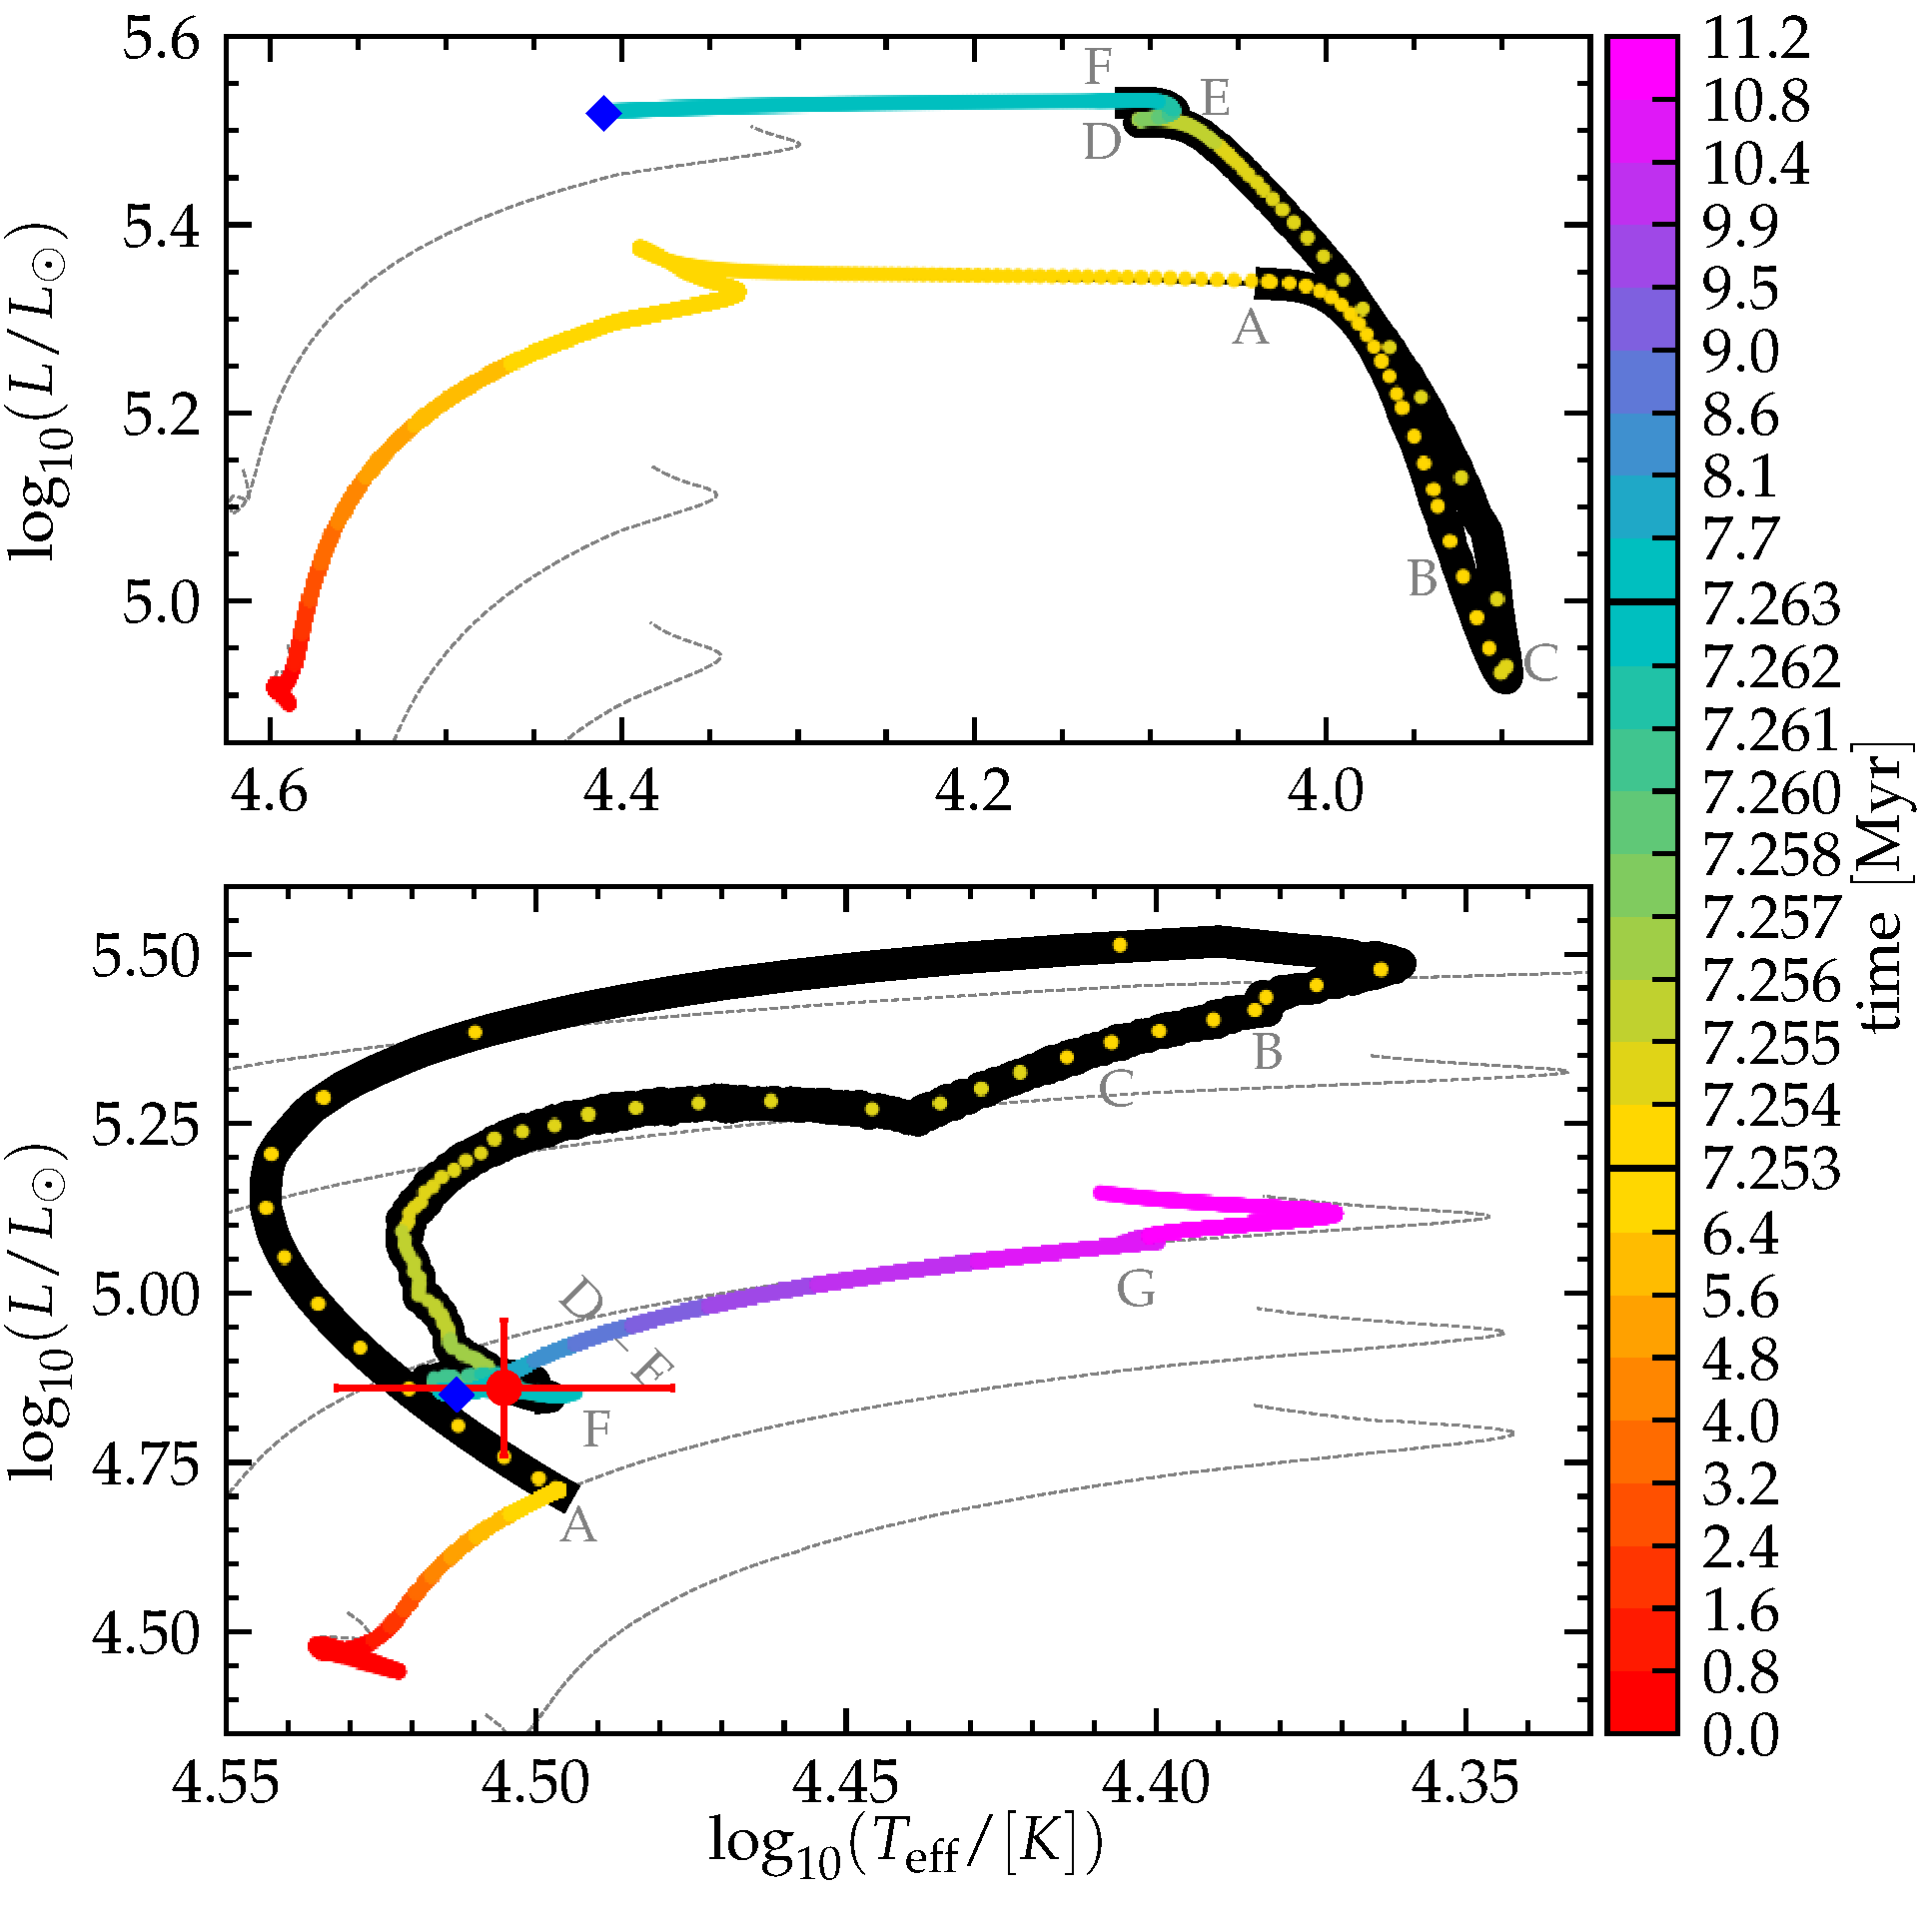
\includegraphics[width=0.5\textwidth]{HRD_colored}
  \caption{HR diagram for the donor star (top) and accretor star
    (bottom) of the progenitor binary of \zoph. Each point is
    separated by 50\,years, and the black outline corresponds to the
    RLOF phase. The colors show the age on a non-uniform scale: we use
    smaller time-bins during RLOF
    ($7.25\,\mathrm{Myr}\lesssim t \lesssim 7.26\,\mathrm{Myr}$).  The
    red data point shows the position of \zoph\ according to
    \citetalias{villamariz:05}, and the blue diamonds mark the end of
    the binary run. We continue the accretor evolution as a single
    star from there until TAMS, thus the bottom panel
    shows a longer time. We emphasize the different scales on the two
    panels. The thin gray dashed line show the main sequence evolution
    of non-rotating single stars of 15, 17, 20, 25, and 30\,$M_\odot$
    at $Z=0.01$ for comparison.}
  \label{fig:HRD_both}
\end{figure}

We describe here the evolution of a binary system in which the
accretor can broadly reproduce the observed features of \zoph. We
assume initial masses $M_1=25\,M_\odot$, $M_2=17\,M_\odot$, and initial
period $P=100$\,days (corresponding to a separation
$a\simeq314\,R_\odot$) with a metallicity of $Z=0.01$.

\Figref{fig:HRD_both} shows the Hertzsprung-Russell (HR) diagrams of
both stars, the donor and accretor are shown separately on the top and
bottom panel, respectively (see \Figref{fig:sp_test} for a single HR
diagram with both stars). Each marker in the figure
corresponds to an elapsed interval of 50\,years in physical time.

After $7.24$\,Myr, the most massive star in the system
 evolves off the main sequence and $\sim{}8400$\,years later, at
point A in \Figref{fig:HRD_both}, it overfills its Roche lobe and starts to donate mass. This
results in a stable case B RLOF on a thermal timescale from point A to
F (black outline of the curves).
We refer to \cite{gotberg:17, klencki:20, laplace:21,
blagorodnova:21} and references therein for a detailed description
of the evolution of massive donor stars in binaries.  Although our
models are more massive, the qualitative behavior of the donor star
is similar. Minor differences might arise because of mixing above
and in the H-burning shell \citep[e.g.,][]{schootemeijer:19,
klencki:21}, and its interplay with the mass transfer.

% Point A - B
At the onset of RLOF (point A in \Figref{fig:HRD_both}), the accretor
star is still on the main sequence with
$T_\mathrm{eff}\simeq10^{4.5}$\,K and its central mass fraction of
hydrogen is $X(^1\mathrm{H})\simeq 0.42$. The accretion of material
drives the star out of thermal equilibrium and it quickly becomes
over-luminous to radiate away the excess internal energy. The accretor
reaches
$L\simeq10^{5.5}\,L_\odot\gg L_\mathrm{nuc}\simeq 10^{5.1}\,L_\odot$,
with $L_\mathrm{nuc}$ the total energy released per unit time by
nuclear burning (integrated throughout the star). However, the
duration of this phase is only $\lesssim 2\times 10^3$\,years,
corresponding roughly to the thermal timescale of the outer envelope
of the accretor. During the same phase, the radius of the
accretor increases dramatically from $\sim7.5\,R_\odot$ to
$\sim35\,R_\odot$.

% Point B - C
At point B -- roughly corresponding to the lowest $T_\mathrm{eff}$ --
the accretor reaches critical rotation, which briefly decreases the
efficiency of mass transfer. This allows the star to contract, and
increase its $T_\mathrm{eff}$. The contraction also increases
$\omega_\mathrm{crit}$, allowing for further accretion to resume.

% Point C - D
At $T_\mathrm{eff}\simeq 10^{4.42}$\,K, slightly after point C, the
inner layers of the donor's envelope are exposed. These layers were
part of the donor's convective core earlier on, before it receded in mass
coordinate. Therefore the transferred material becomes progressively
more He-rich and CNO-processed. The difference in composition of the
incoming material affects the opacity and mean molecular weight in the
outer layers of the accretor and causes a kink in its evolutionary
track. Specifically, material with a high mean molecular weight $\mu$
is placed on top of the comparatively low-$\mu$ primordial envelope of
the accretor. % Point D-F
Because of the increasing gradient in mean molecular weight,
thermohaline mixing starts in the outer layers of the accreting star,
and, together with rotational mixing, it progressively dilutes the
surface $^4\mathrm{He}$ and $^{14}\mathrm{N}$ mass fractions (we
discuss further mixing processes and the internal composition of the
accretor in \Secref{sec:mixing}).  The numerical treatment of these
mixing processes in this regime causes noisy features from point D
to F on the HR diagram of the accretor \citep[e.g.,][]{cantiello:07}.

From D to E the donor star
briefly expands again: by point D the surface is He-rich, and partial
recombination of $^4\mathrm{He}$ drives a convective layer which is extremely thin
in mass ($\lesssim 10^{-4}\,M_\odot$) but can expand to significantly
large radii\footnote{With previous \texttt{MESA} releases, we found it
  challenging to compute models beyond this phase: the large
  increase in radius impacts significantly the mass transfer rate.}.


We emphasize that our adopted (standard) choices to model mixing and
rotation are likely to impact the morphology of the accretor's
evolutionary track during RLOF. The entire duration of RLOF from A to
F is only about $10^4$\,years - of the order of the thermal timescale
of the donor star. Moreover, the accretor spends most of this time
close to the final, post-RLOF position (blue diamond in the bottom
panel). Therefore, observation of a (population of)
mass-transferring binary(ies) is unlikely to provide a direct probe of
the accuracy of our mixing treatment.

\subsection{Mass, velocity, photometry, and age of \zoph\ are naturally
  explained by binary interactions}

The mass and orbital velocity of our accretor star model agrees well
with the measured values for the presently single O-star \zoph.  At
the end of our binary evolution, well after the donor detaches from
its Roche lobe (blue diamonds in \Figref{fig:HRD_both}) the accretor
is a H-rich fast-rotating star of $\sim{}20.1\,M_\odot$.  This matches
well with the estimates for \zoph, which although highly uncertain,
typically include $20\,M_\odot$ in their range (e.g.,
\citealt{hoogerwerf:01}, \citetalias{villamariz:05},
\citealt{neuhauser:20}).

The post-RLOF orbital velocity of the
accretor is $v_2\simeq52\,\kms$. In the subsequent evolution, wind
mass loss from both stars will widen the binary and decrease the
orbital velocity of the accretor star.  As a test, we evolved one
binary assuming the \cite{nugis:00} wind mass loss rate for the
stripped donor until its He core depletion.  At that point the
accretor star's orbital velocity has decreased to $\sim{}40\,\kms$,
and it is expected to decrease even further during the remaining
evolution. The precise amount of the orbital widening and decrease of
the accretor's orbital velocity depends on the very uncertain stripped
star mass loss rate \citep[e.g.,][]{vink:17, sander:20}. Nevertheless,
the value we obtain is in broad agreement with estimates of the
observed runaway velocity of \zoph.

Accounting for both wind mass loss and the amount of mass transferred,
at the end of our binary run (blue diamonds in \Figref{fig:HRD_both})
the donor becomes a He star of $\sim{}9.4\,M_\odot$, likely to
contract further. Depending on its wind mass-loss rate, the stripped
donor's spectrum might show absorption lines, emission lines, or a
mixture of both \citep[e.g.,][]{crowther:07, neugent:17,
  gotberg:18}. It's surface H mass fraction is $\lesssim 0.2$ and even
this residual H-rich layer might possibly be removed by further wind
mass loss \citep[e.g.,][]{yoon:17, gotberg:17, laplace:20}.

In the evolution beyond the blue diamond in \Figref{fig:HRD_both}
(computed as a single star) the accretor settles on a main-sequence
track at higher luminosity compared to the original track because of
the accretion of mass, and its slope is slightly steeper due to the
close-to-critical rotation and the accretion of partially nuclear
processed (He- and N-rich) material.

The effective temperature, bolometric luminosity, and kinematic age of
\zoph\ are also reasonably well reproduced by our model (cf.~\Figref{fig:HRD_both}). After
detachment, the donor star has approximately 0.5 Myr left until
core-collapse, which likely will disrupt the binary system and eject
the accretor star \citep[e.g.,][]{renzo:19walk}. As seen by the colors
of the track in \Figref{fig:HRD_both}, our accretor model spends
around 2\,Myr within the error bars for \zoph\ estimated by
\citetalias{villamariz:05}. This means that after the donor explodes,
the accretor star will look similar to \zoph\ for around 1.5 Myr, in
good agreement with the kinematic age of $1.78\pm0.21$ Myr for \zoph\
\citep{neuhauser:20}.

Moreover, according to our model, the
present-day age of \zoph\ is $\sim 9.5$\,Myr.  The age of the parent
association of \zoph, Upper-Centaurus-Lupus, is relatively uncertain,
with estimates from pre-main sequence isochrone fitting of about
$9\pm1$\,Myr, but an average age of $15\pm3$\,Myr
\citep[][]{pecaut:16}.  Given the sensitivity of our model to
rejuvenation (see \Secref{sec:mix_comparison_single}), the large age
scatter of the region, and the unknown systematics in age
measurements, we consider our model broadly compatible with the
existing constraints.

We discuss in detail the mass and mass-transfer evolution in
\Secref{sec:MT}, the internal and surface rotation in
\Secref{sec:rot}, and the chemical composition in
\Secref{sec:mixing}. As a summary, the accretor in our binary starts
with 17$\,M_\odot$ and accretes about 3.4\Msun\ material during mass
transfer (out of $\sim 10.6$\Msun\ total transferred). This causes
rejuvenation, and our accretor reaches TAMS 11.2\,Myr. For comparison, the
lifetime of a non-rotating single star of 17\,$M_\odot$ is
$\sim$11.1\,Myr, while the initially 20\,$M_\odot$ rotating models
have a main-sequence lifetime of $\sim$9.2-9.6\,Myr (longer for higher
initial rotation rates). After mass the mass transfer, the accretor
star spins rapidly (see \Secref{sec:surf_rot}), and its surface
composition is determined by the accretion of material from the
donor's core progressively mixed inwards (see
\Secref{sec:surf_comp}). We find that the rotation and surface
composition of \zoph\ are more easily explained by accretor models
than single rotating stars (e.g., \citetalias{villamariz:05}).

\section{Mass and mass transfer rate evolution}
\label{sec:MT}

\begin{figure}[bp]
  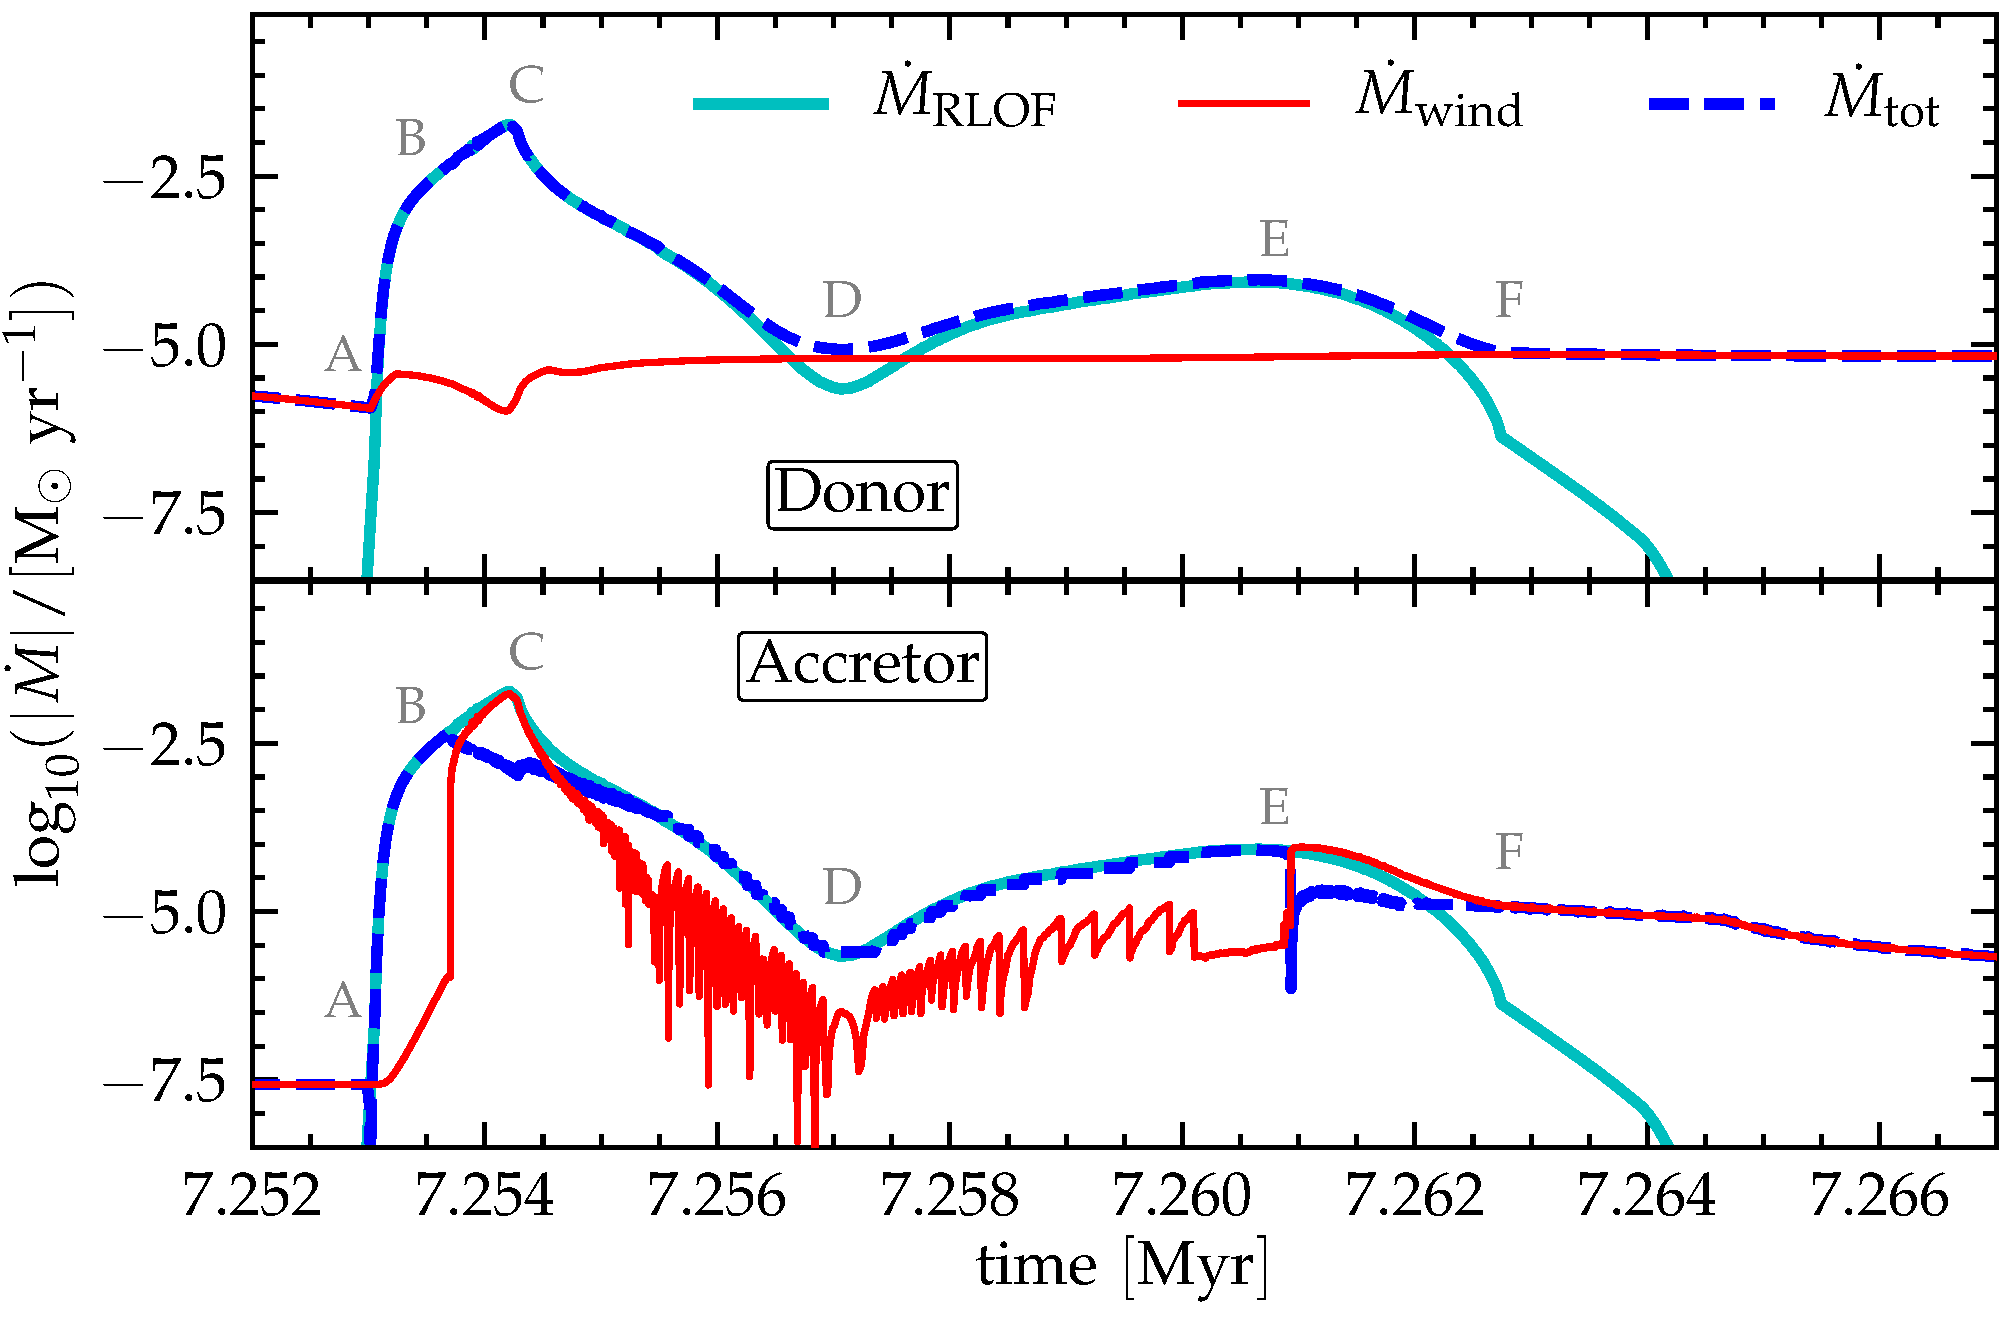
\includegraphics[width=0.47\textwidth]{MT}
  \caption{The top panel shows the total mass of each star as a
    function of time during RLOF. The middle and bottom panel show the
    contributions to the rate of mass change for the donor and
    accretor star, respectively. The cyan solid lines show the mass
    transfer rate due to RLOF, the red lines show the (mechanically
    enhanced) wind mass loss rates. In the middle panel, the dashed
    blue lines shows their sum, corresponding to the total mass loss
    rate of the donor. During RLOF the accretor reaches critical
    rotation, which leads to oscillations in the
    rotationally-enhanced wind mass loss.}
  \label{fig:MT}
\end{figure}

\Figref{fig:MT} shows the mass evolution (top panel) and the rate of
mass change (middle and bottom panels) for each individual star during
the mass transfer phase. The donor star (middle panel) loses mass via
RLOF ($\dot M_\mathrm{RLOF}<0$, cyan line) and wind
($\dot M_\mathrm{wind}<0$, thin red line). The dashed blue line shows
the sum of these two negative terms and represents the total rate of
mass change of the donor. Conversely, the accretor (bottom panel)
gains mass via RLOF (i.e., $\dot M_\mathrm{RLOF}>0$ from the
accretor's point of view), but still loses mass to the wind
($\dot M_\mathrm{wind}<0$).
At peak (point C), the mass transfer rates
reaches values above $10^{-2}\,M_\odot\ \mathrm{yr^{-1}}$ and taps
into the optically thick matter of the donor (i.e., the donor's Roche
radius becomes smaller than its photosphere $R_\mathrm{RL,1}<R_1$).

Initially, between point A and B, the mass transfer rate equals the
mass accretion rate (bottom panel of \Figref{fig:MT}), that is
initially the accretion is (by construction) fully conservative. The
bulk of the mass -- $\sim{}2\,M_\odot$ out of
$\sim{}3.1\,M_\odot$ -- is accreted during this initial phase, which
lasts about $\sim{}2\times10^3$\,years. As the mass and surface
rotation rate of the accretor increase, the assumed
rotational-enhancement of the wind progressively increases the
mass-loss rate by $\sim$5 orders of magnitude. The
mechanically-enhanced wind controls the accretion efficiency, and at
$\sim{}7.254$\,Myr (from B to C, where the red solid line and the cyan
line overlap) the mass transfer becomes briefly non-conservative. In
our setup, the majority of the mass transferred during this phase is
ejected as a fast wind from the accretor, carrying the same specific
angular momentum as the orbit of the accretor star. The decreased
accretion efficiency allows, the accretor to contract (point B to C,
cf.~\Figref{fig:HRD_both}).  In the remaining evolution from C to F,
the interplay between the wind mass loss rate, the spin-up due to
accretion and the spin-down due to inward transport of angular
momentum (see \Secref{sec:rot}) cause large oscillations in the wind
mass loss rate. Nevertheless, for most of the evolution, accretion
still occurs, albeit not-fully conservatively. This allows for
CNO-processed material from the donor to reach the surface of the
accretor during late stages of mass transfer.

The minimum of the mass transfer rate in point D corresponds to a
brief phase of contraction (see also \Figref{fig:HRD_both}). However,
from D-E, the donor star expands again.  This is due to the
partial recombination of the now He-rich outer layers, which causes a
transient surface convection layer. The convective layers expand,
leading to an increase in the mass-transfer rate, despite at this
point % the donor is less massive than the accretor and
the binary %orbit
is widening. During this phase, the mass transfer becomes highly
non-conservative again (in the bottom panel the wind and the mass
accretion rate nearly cancel each other again at $\sim7.261$\,Myr),
until the donor completely detaches from its Roche lobe at point F.


\section{Rotation and angular momentum transport in the accretor}
\label{sec:rot}

\subsection{Surface rotation}
\label{sec:surf_rot}

\begin{figure}[tbp]
  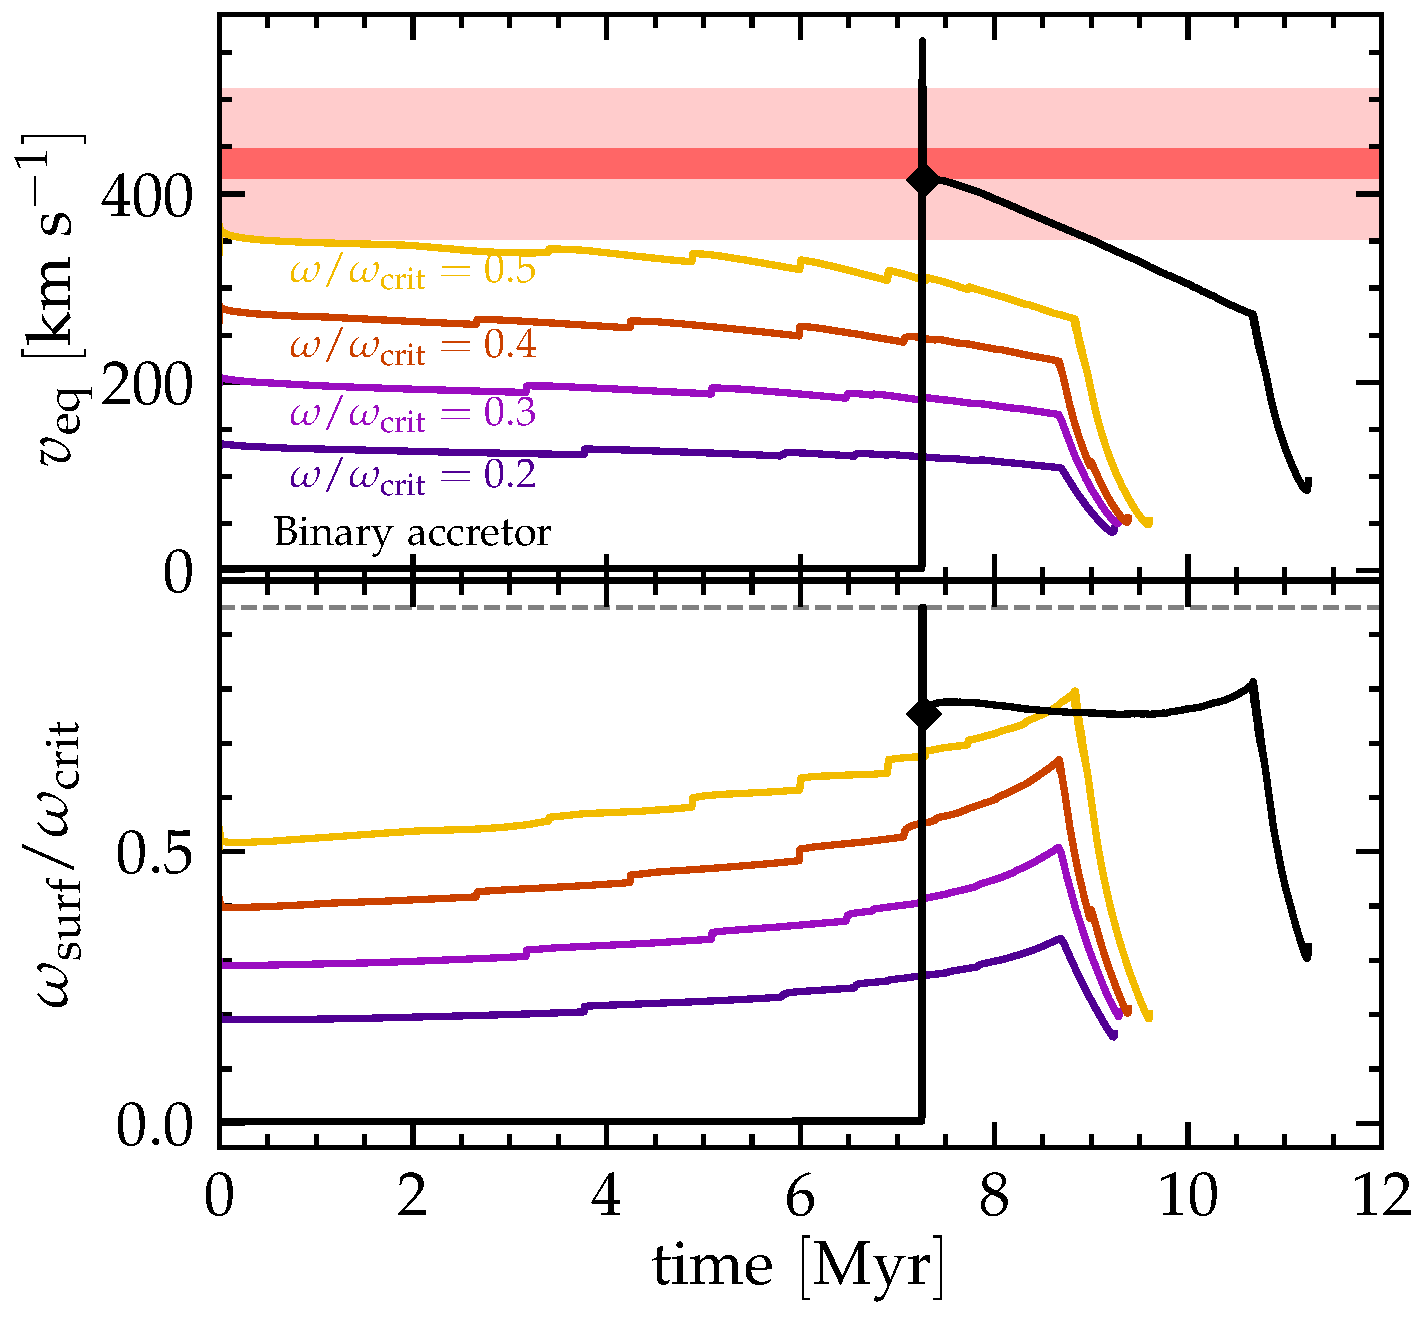
\includegraphics[width=0.5\textwidth]{zeta_rot}
  \caption{Equatorial surface rotational velocity (top panel) and
    $\omega/\omega_\mathrm{crit}$ (bottom panel) for the accretor
    model (black) and single rotating $20\,M_\odot$ stars (colored
    lines). The red bands in the top panel correspond to the
    $v\sin(i)$ observed for \zoph\ (see text). At $\sim{}7.25$\,Myr
    the mass transfer quickly spins up the accretor to critical
    rotation: the dashed horizontal line in the bottom panel shows the
    upper-limit we impose. By the time the donor detaches from the
    RLOF the accretor is still spinning at $\sim{}400\,\kms$. From
    this point (diamonds) onwards, we continue the evolution as a
    single star, and the accretor spins down because of wind mass
    loss.  Note however that we use the wind mass-loss rate from
    \cite{vink:01}, which might be $\sim$2 orders of magnitude too
    high for \zoph\ \citep{marcolino:09}.}
  \label{fig:surf_rot}
\end{figure}

Rapid rotation is one of the main properties expected as a result of
spin up due to mass accretion \citep{packet:81}.  One of the main
distinguishing features of \zoph\ is its extremely high surface
rotation rate.  The black line in the top panel of
\Figref{fig:surf_rot} shows the evolution of the surface equatorial
rotational velocity $v_\mathrm{eq}$ for our accretor model, not
including any projection effect. More precisely, $v_\mathrm{eq}$ is a
mass-weighted average of the rotational velocity of layers with
opacity $\tau\leq 100$. The dark horizontal red band corresponds to
the $v\sin(i)=432\pm16\,\kms$ measured for \zoph\ by \cite{zehe:18},
and the lighter band shows a range of 5 times their error bar, which
roughly encloses the majority of the estimated $v\sin(i)$ for \zoph\
in the literature
$350\,\kms\lesssim v\sin(i)\lesssim 600\,\kms$ (e.g.,
\citealt{gordon:18} and \citealt{walker:79}, respectively).  For comparison, the colored solid lines show also
$v_\mathrm{eq}$ for models of rotating
$20\,M_\odot$ single stars with birth spins of $\omega/\omega_\mathrm{crit}
=
0.2$, 0.3, 0.4 and 0.5. The bottom panel of \Figref{fig:surf_rot} shows instead the ratio of the surface rotational frequency
$\omega_\mathrm{surf}$ to the critical rotational frequency $\omega_\mathrm{crit}$.

The initial binary is wide enough that assuming tidal synchronization
at ZAMS implies a very low $v_\mathrm{eq}\lesssim 3\,\kms$. At 7.25\,Myr, mass transfer rapidly spins
up the accretor to critical rotation,
$v_{\rm crit}\sim{}520\,\kms$. This corresponds to
$\omega/\omega_\mathrm{crit}\simeq 0.95$ (dashed horizontal line in
the bottom panel of \Figref{fig:surf_rot}), which is the upper-limit
we impose in our models (see \Secref{sec:methods}).

The star remains fast rotating throughout the mass transfer phase, and
the remaining evolution in a binary which ends at the black diamond in
\Figref{fig:surf_rot} (corresponding to the blue diamonds in
\Figref{fig:HRD_both}). In the remaining evolution, the star spins
down progressively through wind mass loss, and within $\sim$2\,Myr its
averaged surface rotational velocity drops below $\sim{}350\,\kms$.

Both the single star models and our accretor (after being spun up)
evolve to higher $\omega/\omega_\mathrm{crit}$ because of the increase
in stellar radii and corresponding decrease in $\omega_\mathrm{crit}$
\citep[e.g.,][]{langer:98, zhao:20}. However, our accretor model
remains at a higher
$\omega_\mathrm{surf}/\omega_\mathrm{crit}\simeq 0.75$ for a
significantly longer time: the chance of observing a single rotating
star at very high $\omega_\mathrm{surf}/\omega_\mathrm{crit}$ is lower
than for an accretor from a massive binary system. Moreover,
$\omega_\mathrm{surf}/\omega_\mathrm{crit}$ we find is in good
agreement with the observationally constrained values for typical Oe
and Be stars \citep[see][for a review]{rivinius:13}.

Close to the end of the main sequence, the increase in wind mass loss
rate as the stars cross the bistability jump \citep[due to iron recombination
at $T_\mathrm{eff}\simeq25\,000\,\mathrm{K}$, e.g.,][]{vink:00}
strengthens the surface spin-down. This effect is also seen in the
late main-sequence evolution of single stars rotating rapidly at
birth.

\Figref{fig:surf_rot} shows that our model retains a significant
surface rotation for a long period of time, comparable to the
kinematic age of \zoph. Since the spin up of the accretor happens
roughly half-way through its main sequence, the star is much faster
rotating than single stars of the same (post-RLOF) mass initialized as
fast rotators at ZAMS. Although \Figref{fig:surf_rot} does not account
for the projection angle, \cite{zehe:18} argued for
$i\geq56$\,degrees, corresponding to an upward shift of the red band
in \Figref{fig:surf_rot} of $\lesssim 20\%$. This shift impacts the
comparison of \zoph\ to our accretor model and to single star models
in the same way.

We emphasize that our model is computed using the \cite{vink:00,
  vink:01} wind mass-loss rate with full efficiency throughout its
evolution. This is two orders of magnitude higher than the wind mass
loss rate reported by \cite{marcolino:09} (weak wind problem,
however, see also \citealt{lucy:12, lagae:21}). While this may impact
the evolution of the binary even before RLOF, it presumably increases the
spin-down rate of our model compared to the observations. We expect
that an accreting star modeled with lower wind-mass loss rate
post-RLOF would retain an even higher surface rotation for longer (see
also \Secref{sec:single_star_uncertainties}).

\subsection{Internal rotation -- comparison to
  single stars}
\label{sec:rot_comparison_single}

\begin{figure*}[tbp]
  \centering
  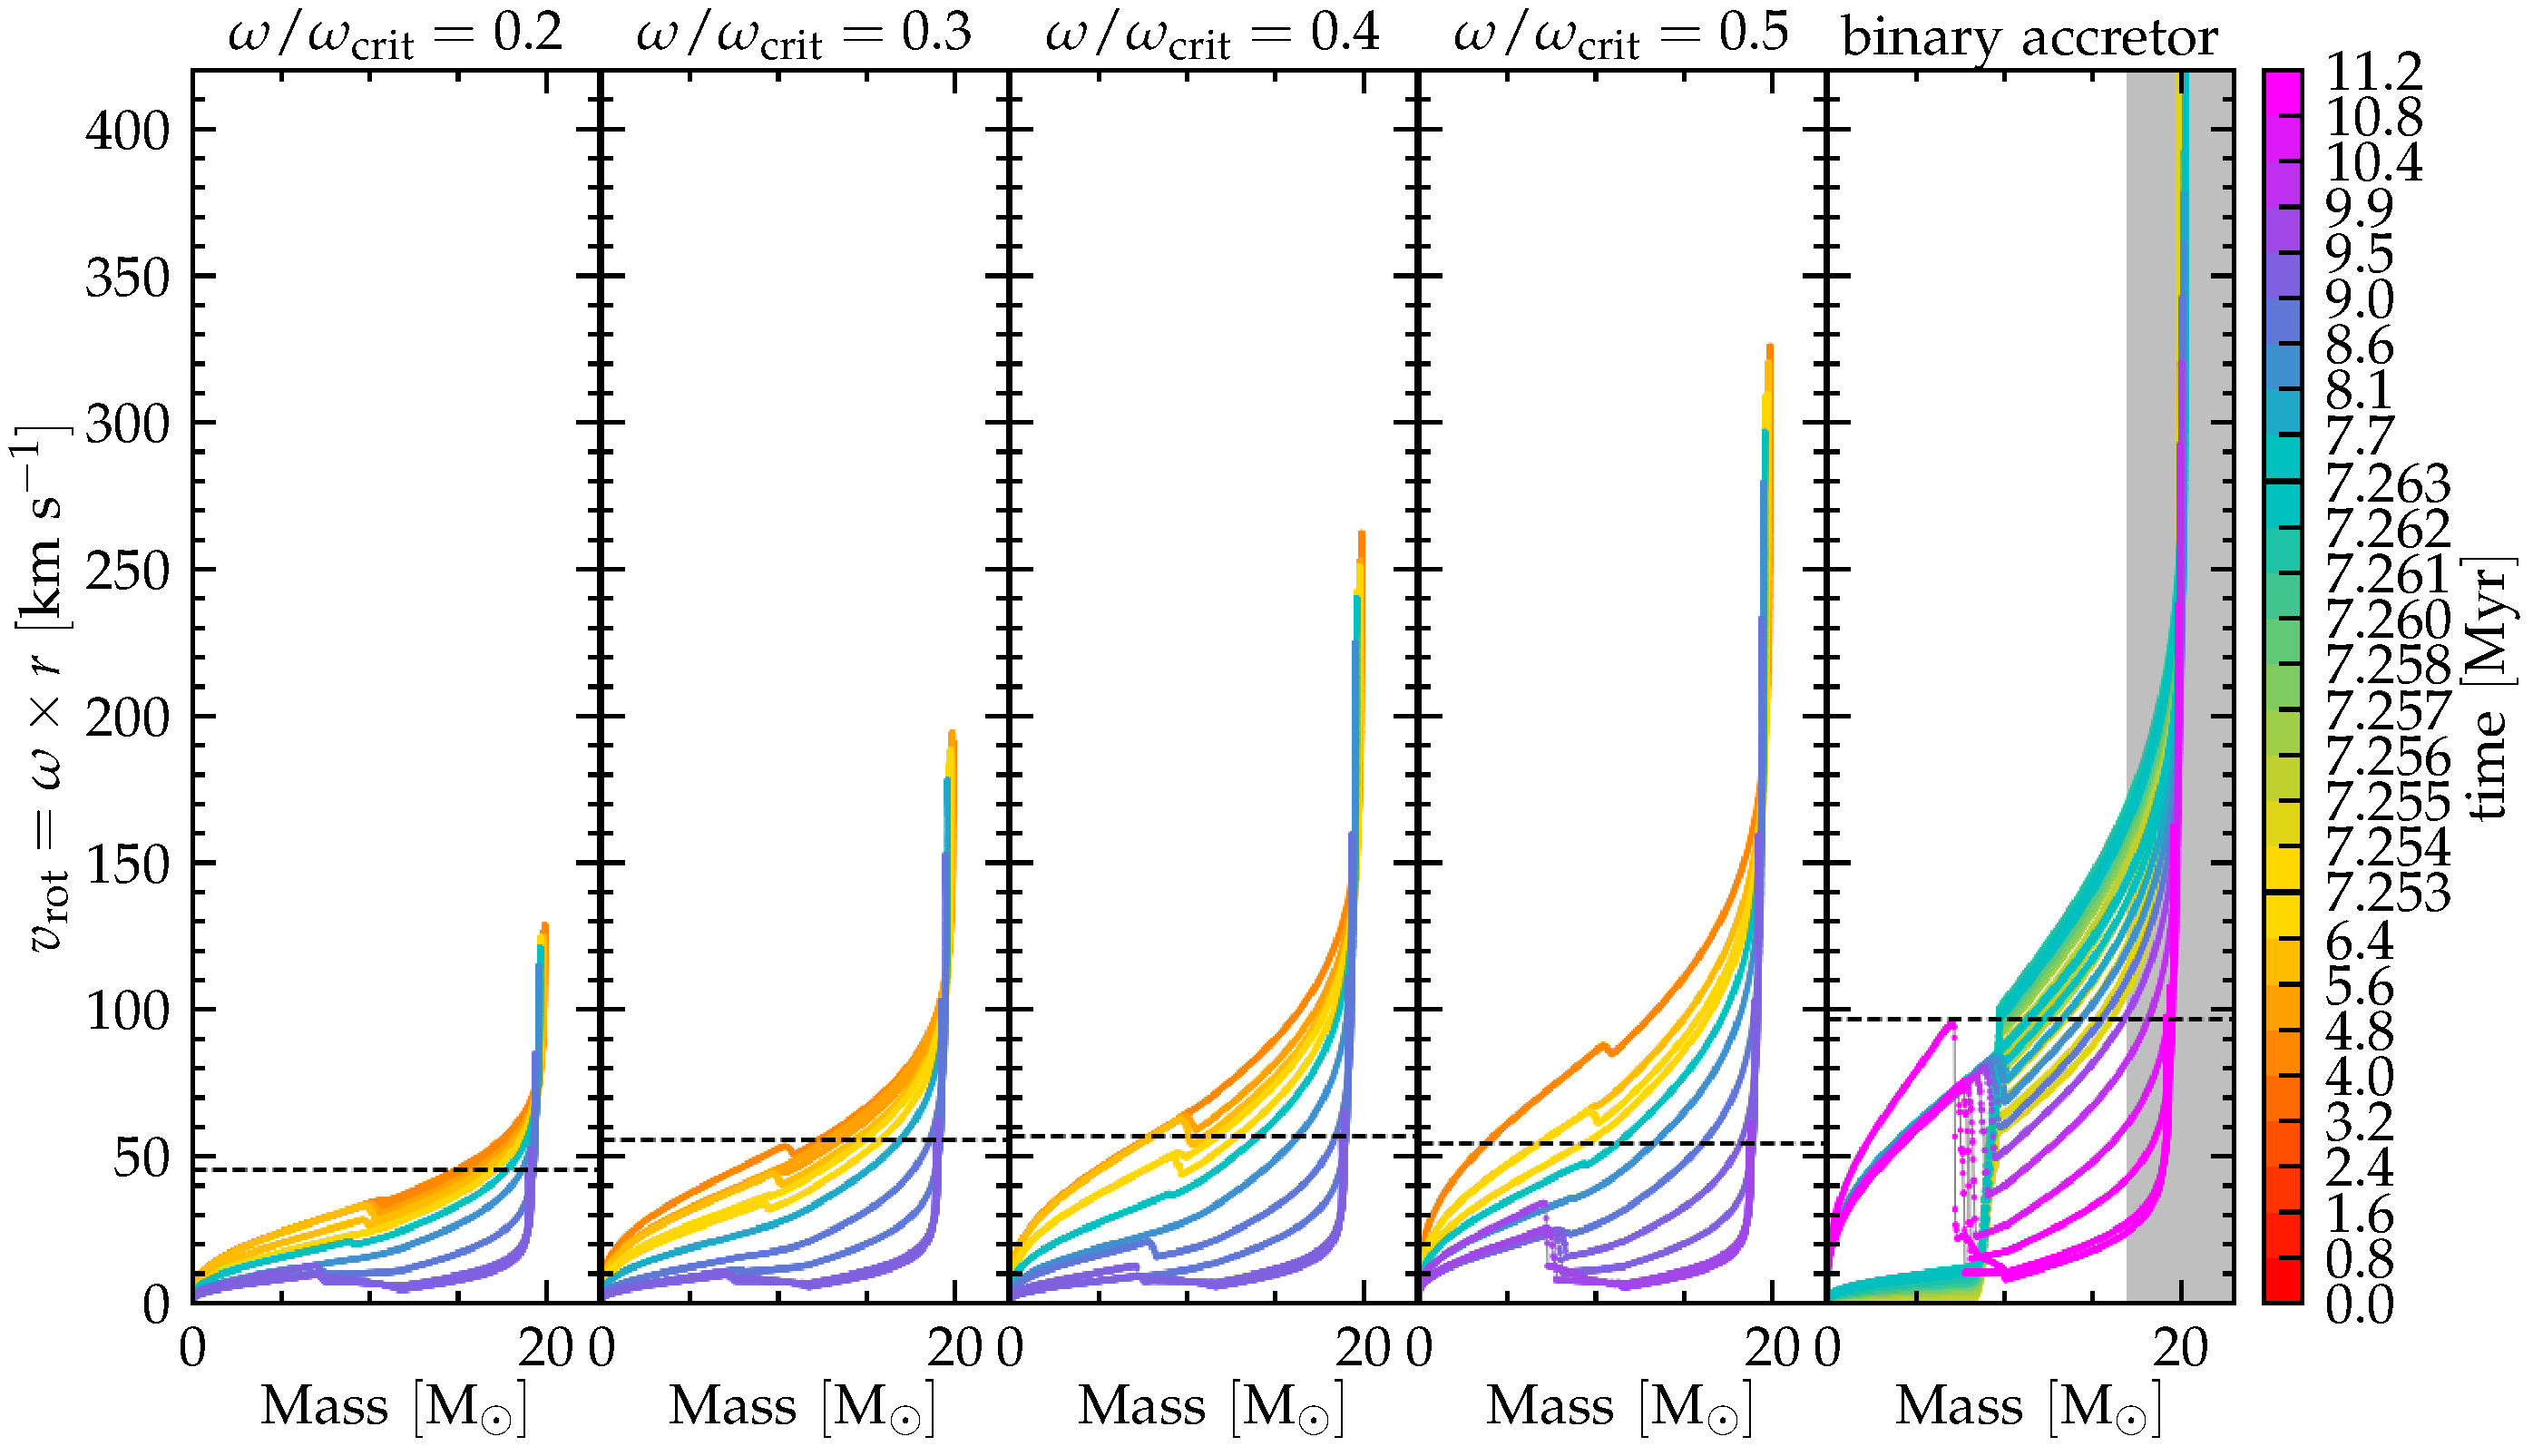
\includegraphics[width=\textwidth]{zeta_Rotational_struct_colored}
  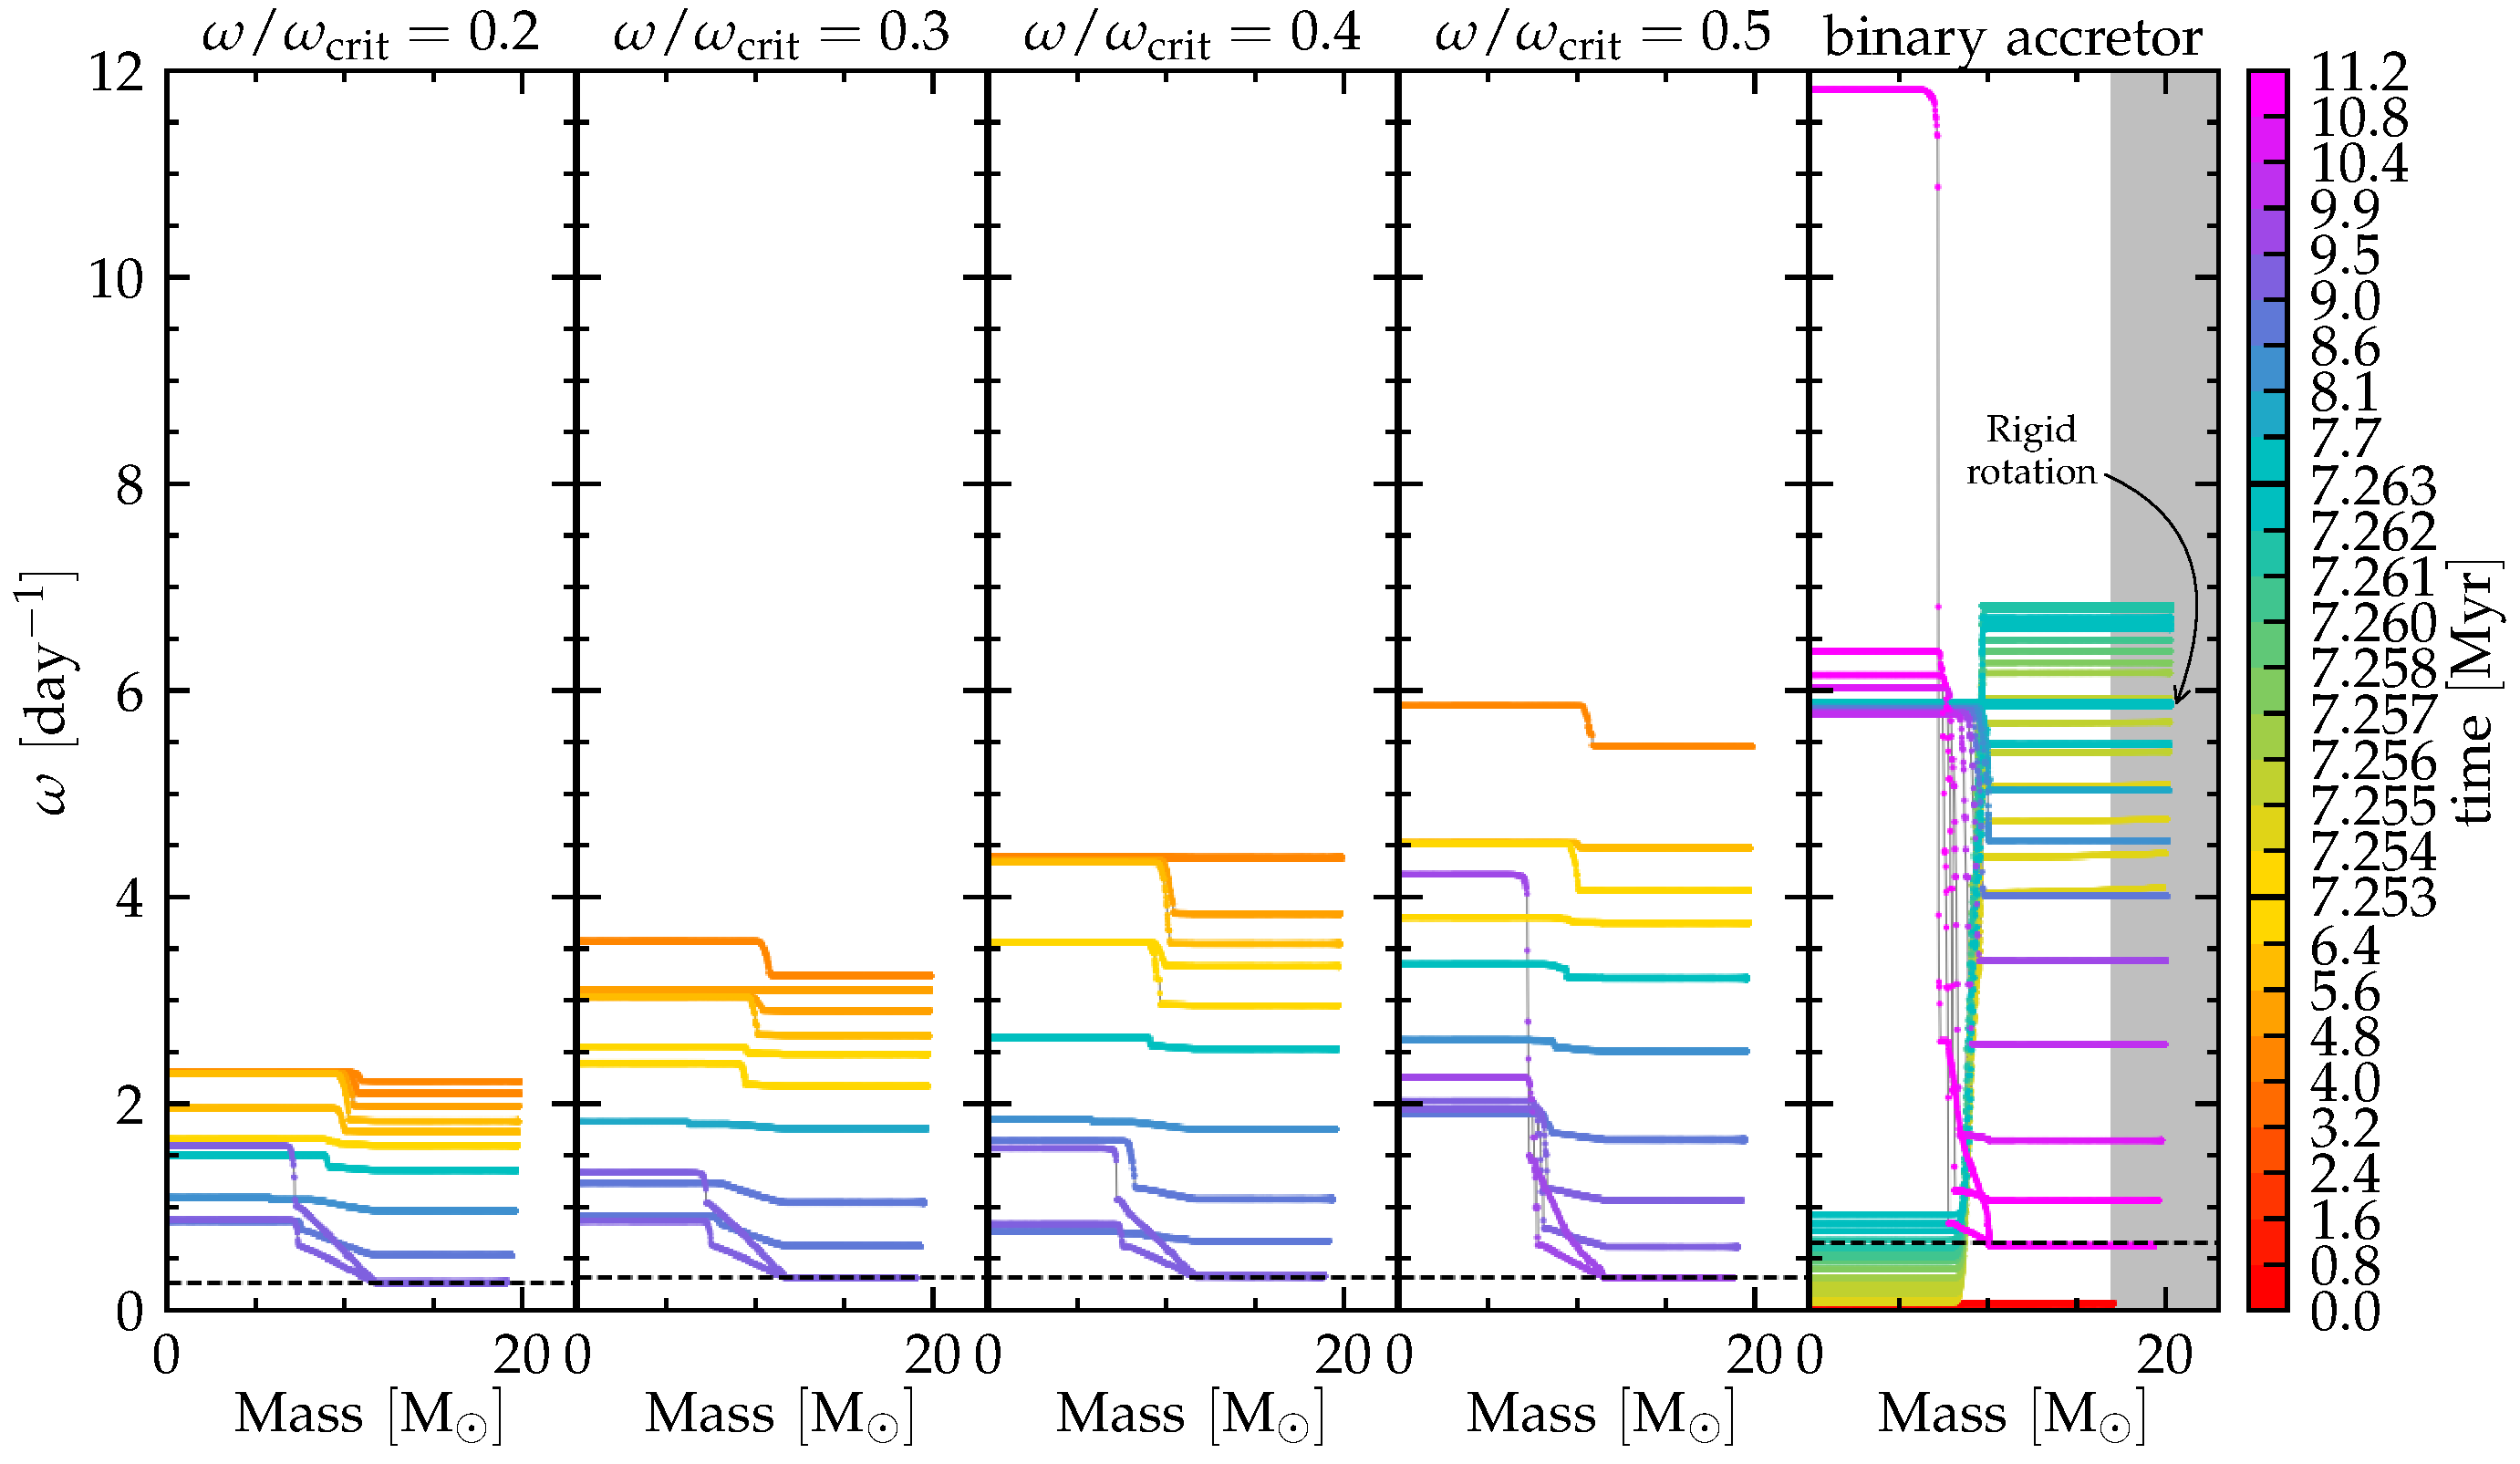
\includegraphics[width=\textwidth]{omega_struct_colored}
  \caption{Top: Internal rotational profile for $20\,M_\odot$ single
    star models with increasing $\omega/\omega_\mathrm{crit}$ at birth
    (first four panels), and for the accretor of our fiducial
    binary. Bottom: internal rotational frequency profile. As in
    \Figref{fig:HRD_both}, the colorbar is non-uniform. In the top
    (bottom) panel the thin dashed black lines mark the TAMS surface
    rotation rate (surface rotation frequency). In the rightmost
    panels, the gray areas indicate mass accreted during RLOF. The
    pink lines (TAMS) in the last panel show that the core of the
    accretor is rotating almost as fast as its surface despite its
    much smaller radius, and both are faster than the surface of
    single star models.}
  \label{fig:struct_rot}
\end{figure*}


Our model suggests that the internal rotational profile of accretor
stars evolve differently compared to those of rotating single stars.
To illustrate the angular momentum transport in our accretor stars, it
is again helpful to compare with single rotating $20\,M_\odot$
models. Typically, single stars are assumed to be solid-body rotators
at ZAMS \citep[e.g.,][]{maeder:00}.
% As they contract and lose mass, their internal rotational
% profile evolves differently than the profile obtained spinning up the
% secondary star later on, from its surface, and to
% critical rotation.

The top row of \Figref{fig:struct_rot} shows the internal rotational
velocity, $v_\mathrm{rot}=\omega\times r$, while the bottom row shows
the angular frequency profile $\omega$ as a function of mass
coordinate. The first four panels in each row show single rotating
stars with increasing initial $\omega/\omega_\mathrm{crit}$, the last
panels shows the accretor model.  The gray area in the rightmost
panels highlights matter accreted during RLOF, while the colors of the
lines indicate the age of the star at each profile shown.

The thin black horizontal dashed lines in each panel of the top row of
\Figref{fig:struct_rot} mark the TAMS surface rotation rates: all our
single star models reach a TAMS surface
$v_\mathrm{rot}\simeq50-60\,\kms$. Initially faster rotating models
spin down more in their outer layers, have slightly longer main
sequence lifetimes (because of rotational mixing increasing the
available fuel), and develop stronger differential rotation. As the
core contracts and spins up, the single star profiles show the
progressive development of a core-envelope interface.

Conversely, the entire interior of the accretor has a negligible
rotational velocity until RLOF (starting at
$\sim{}7.25$\,Myr). Because of binary mass transfer, the accretor is
spun up from the surface inwards, late in its evolution, and it
reaches critical rotation $\omega/\omega_\mathrm{crit}\simeq1$. In our
model, inward transport of angular momentum creates a $v_\mathrm{rot}$
profile monotonically decreasing from the surface to the center. After
the end of mass transfer, roughly at $7.27$\,Myr, the accretor
achieves rigid and close to critical rotation (flat profiles in the
last panel on the bottom row of \Figref{fig:struct_rot},
$\omega \sim 6$ day$^{-1}$). At the end of our binary run the
accretor is still rigidly rotating, which persists\footnote{To calculate
  the duration, we consider rotation to be rigid if the difference
  between the minimum and maximum frequency throughout the star is
  $\Delta \omega \lesssim 10^{-2}\,\mathrm{days^{-1}}$.} for a total
duration of $\sim10^{4}$\,years. Afterwards, the accretor's envelope
spins down because of winds and its evolutionary expansion.  By the
end of the accretor's main-sequence, the surface still spins with
$v_\mathrm{rot}\simeq100\,\kms$, which is approximately twice as fast
as the single star models.

Conversely, in the remaining evolution, the core contracts (decrease
in $r$). The weak core-envelope angular momentum coupling provided by
the Spruit-Tayler dynamo leads to an approximately constant total
angular momentum in the core, therefore, as it contracts and decreases
its momentum of inertia, its rotation rate $\omega$ increases
dramatically.  At the end of the main sequence, the outer edge of the
core of the accretor star has a similar rotational velocity as the
surface, and much larger than for the single star models.
Consequently, the TAMS core-envelope interface
for the accretor is much more prominent than for in single rotating
stars. It might be possible to distinguish accretors from
initially single stars by using asteroseismology to measure the core
rotation rate \citep[e.g.,][]{cantiello:14}. However, this requires
the detection of mixed modes which is presently challenging for
massive stars.

Moreover, the higher core spin of accretors may have
important implications for their future explosions
\citep[e.g.][]{macfadyen:99, cantiello:07}, the spin of the
resulting compact objects, and the analysis of gravitational-wave
events \citep[e.g.,][]{zaldarriaga:18, qin:18, callister:21}.

\section{Mixing and composition of the accretor}
\label{sec:mixing}

\begin{figure}[htbp]
  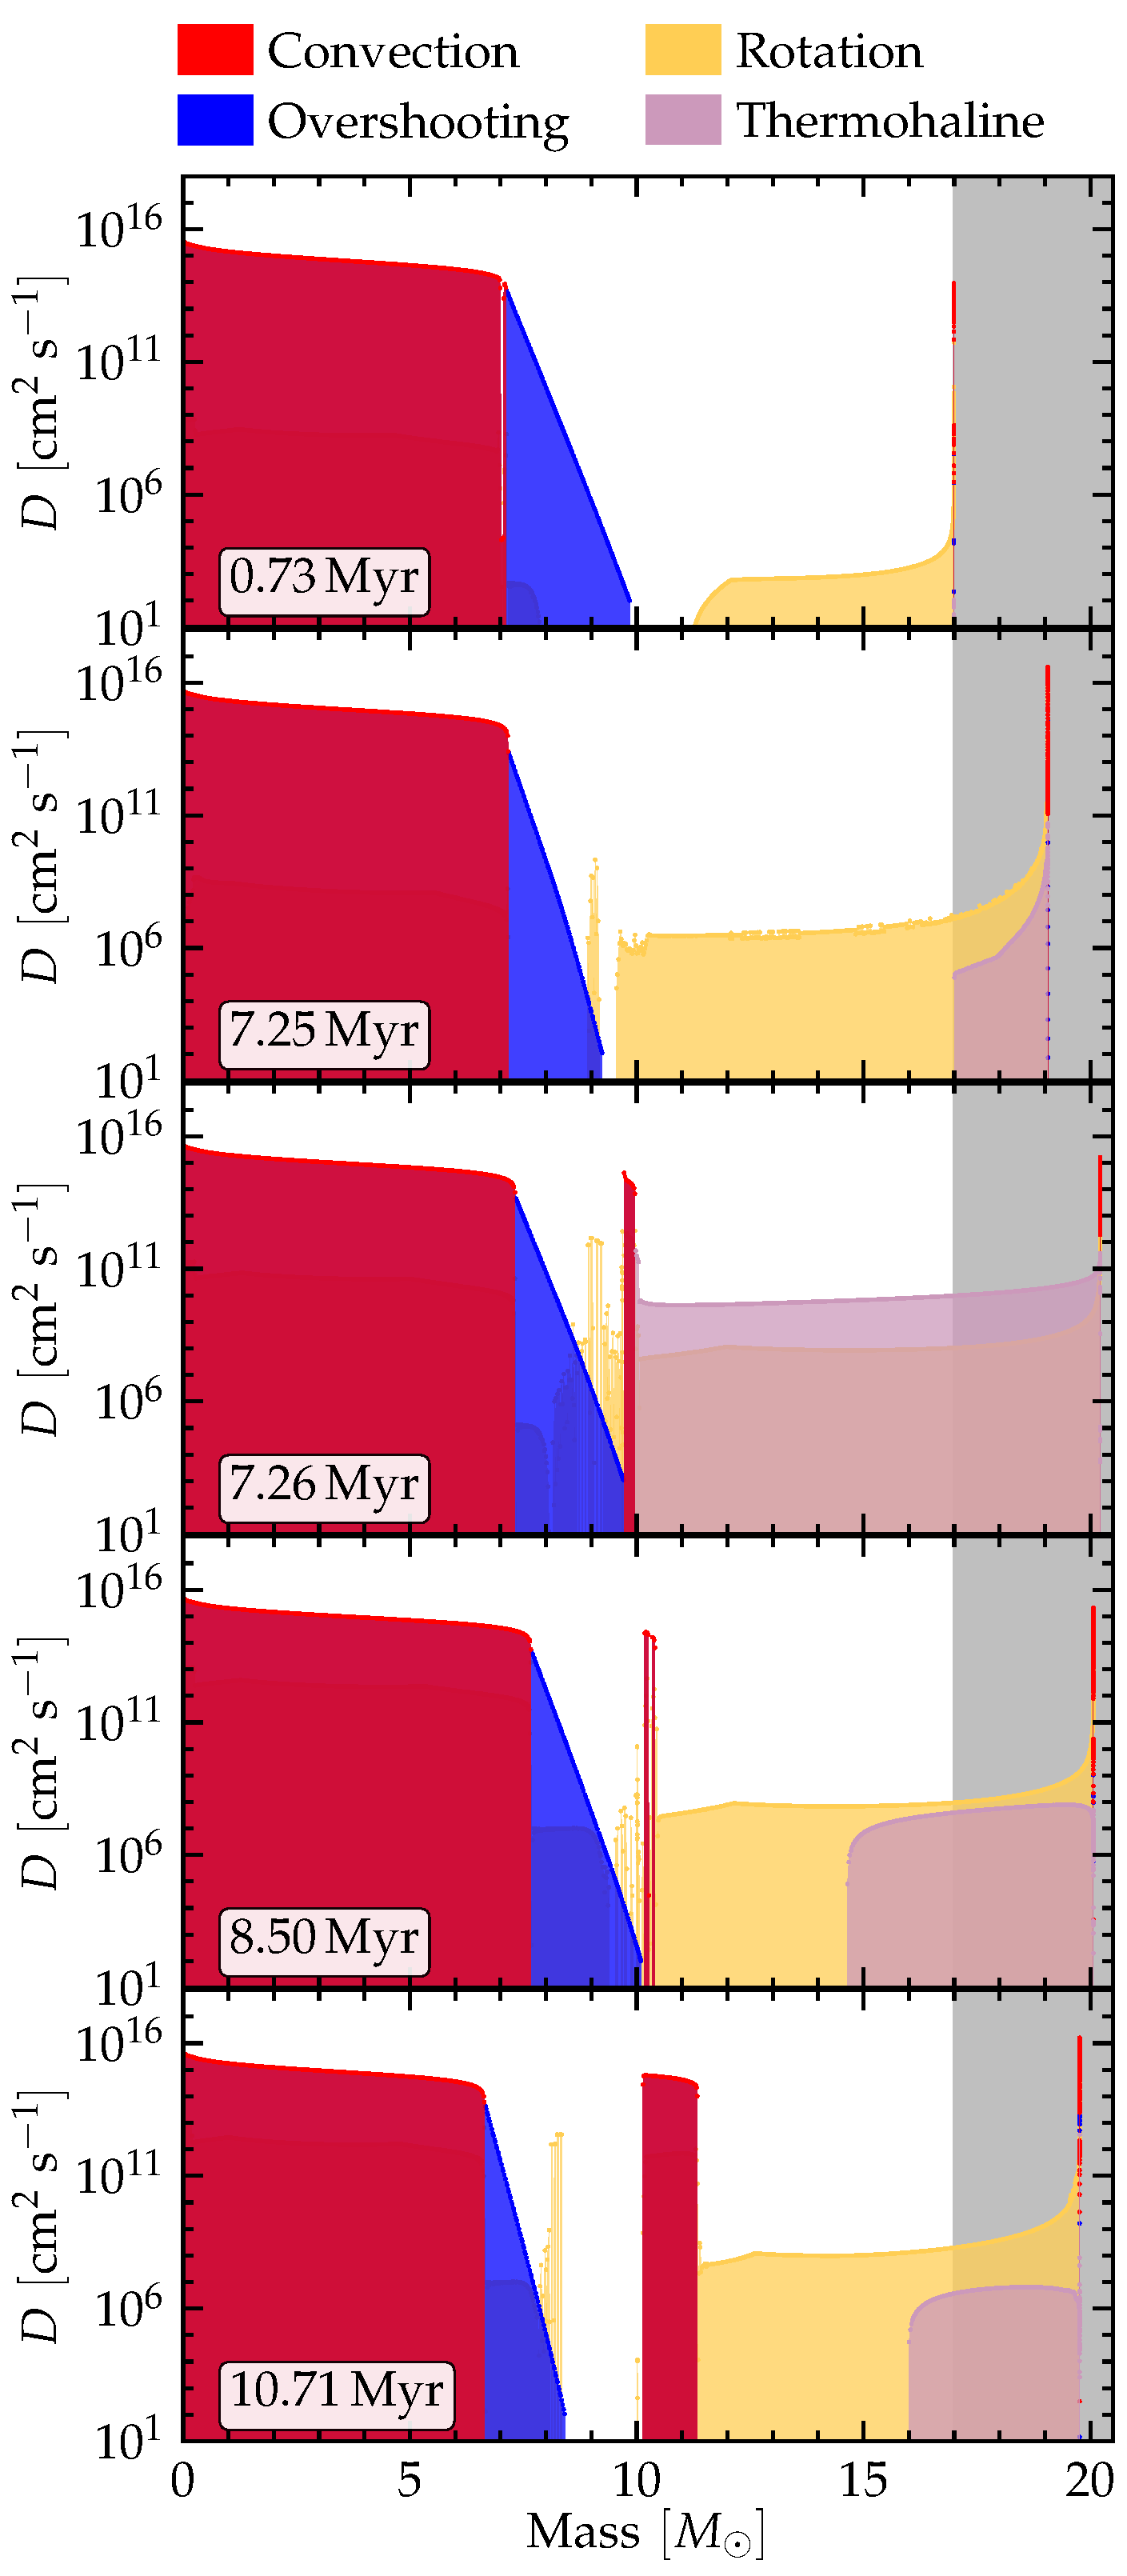
\includegraphics[width=0.47\textwidth]{D_mix_vertical}
  \caption{Mixing diffusion coefficients in the accretor star as a
    function of mass (the center corresponds abscissa 0 and the
    surface to the maximum abscissa for which a diffusion coefficient
    is plotted). The gray area on the right highlights accreted
    material. From top to bottom, each panel shows a profile during
    the main sequence (before point A in \Figref{fig:HRD_both}), early
    during RLOF (close to point C), mid-RLOF (close to point D), late
    during RLOF (between point D and E), and after RLOF (point G). A
    movie of the entire evolution is available at
    \url{https://doi.org/10.5281/zenodo.4701565}.}
  \label{fig:D_mix}
\end{figure}

Rotational mixing and thermohaline mixing induced by mass accretion
affect significantly the composition profile of our accretor star. They both
act primarily in the envelope, starting from the
surface and growing inwards. \texttt{MESA} treats mixing using a
diffusion approximation \citep{paxton:11}, and to illustrate the
dominant processes we show in
\Figref{fig:D_mix} the diffusion coefficients for the mass
fractions of elements as a function of Lagrangian mass coordinate at
selected times. From top to bottom, we show the mixing contribution in
the interior of our accretor star model at:
\begin{itemize}
\item early main sequence before RLOF (i.e., before point A in
  \Figref{fig:HRD_both} and \Figref{fig:MT});
\item early during RLOF (slightly after point C);
\item late during RLOF (close to point F);
\item post-interaction structure (within the red errorbars for \zoph\ in \Figref{fig:HRD_both});
\item close to TAMS (point G in \Figref{fig:HRD_both}).
\end{itemize}
In each panel of \Figref{fig:D_mix}, the gray background highlights
mass coordinates exceeding the initial mass of the star.  The
remaining colors show convection (red), overshooting (blue),
rotational mixing (yellow), and thermohaline mixing (pink). Rotational
mixing includes all the rotational instabilities that we consider --
meridional currents, secular and dynamical shear instabilities, and
GSF instability. However, throughout the evolution rotational mixing
is strongly dominated by the meridional currents (Eddington-Sweet
circulations).  The only exception is at the interface between core
and envelope (i.e., at the outer edge of the overshooting region),
spin-up of the core and subsequently its contraction and spin up (see
\Secref{sec:rot}) can lead to significant dynamical shear (and GSF
mixing to a lesser extent). For clarity, we do not show semiconvection
which never dominates the mixing in our accretor model.

% Main-sequence massive star - before interaction
The top panel shows the typical structure of a main sequence massive
star: the convective core initially reaching $\sim{}7\,M_\odot$ with
the overshooting extension to $\sim{}9\,M_\odot$. The slow initial
rotation causes a weak meridional circulation in the envelope. Meridional
circulations are also present in the core throughout the evolution,
but with a diffusivity more than nine orders of magnitude lower than
core convection. A small sub-surface convective zone is also
appreciable at the very surface (see, e.g., \citealt{cantiello:21}).

% Early during RLOF
In the second panel from the top, the star has already accreted
$\sim{}2\,M_\odot$ (extending in the gray region), including some
CNO-processed material from the inner layers of the core, and its
surface is already spun up to $\sim{}330\,\kms$. Thermohaline mixing
has started in the newly accreted layers, but it is subdominant
compared to rotational mixing due to meridional circulations in the
envelope. Angular momentum transport (by the Spruit-Tayler dynamo) has
already imparted some rotation to the inner layers of the
envelope. This leads to the disconnected spike in rotational mixing at
the outer edge of the core (at mass coordinate $\sim{}9\Msun$),
dominated by dynamical shears.  We note that between the top panel and
the onset of RLOF, the convective core recedes in mass coordinate,
but, by the time shown in the second panel, the accretion of mass has
caused the core to grow back to its initial size.

% Late during RLOF
In the third panel, the star has already accreted all the mass that it
will. Thermohaline mixing takes over the dominant role in the
envelope (although meridional circulations persist behind it, with a
mixing coefficient two orders of magnitude smaller). The core is still
growing in mass, meaning that rejuvenation is still on-going. The
mixing at the core-envelope boundary at $\sim9-10\Msun$ is partially
still due to dynamical shear, but a thin, off-center, convective
region also appears. Because we adopt an exponentially decreasing
overshooting, the diffusion coefficient at the outer edge of the
overshooting region is small, and therefore is the mixing between the
core and the off-center convective region is weak: this off-center
convective region does not inject a significant amount of H-rich
material in the core and is not participating significantly to the
star rejuvenation. We do not include
over/undershooting for off-center convective layers, which could
increase the coupling between these layers.

% Post-interaction
After detachment (the fourth panel in \Figref{fig:D_mix}, roughly
corresponding to \zoph's structure today), thermohaline mixing is
progressively shutting down from inside out, while meridional
circulations remain on.

% At TAMS
Finally, the last panel displaying the interior mixing shortly before
TAMS shows that, as the post-RLOF evolution proceeds, the previously
thin, off-center convective layer grows thicker, including almost
1.5\Msun\ of material between the mass coordinates $10-11.5\Msun$. In
addition, the hydrogen-burning core has receded, leaving a
$\sim 1.5\Msun$ thick layer that is un-affected by mixing, meaning
that the core and the convective layer have disconnected.


\begin{figure}[tbp]
  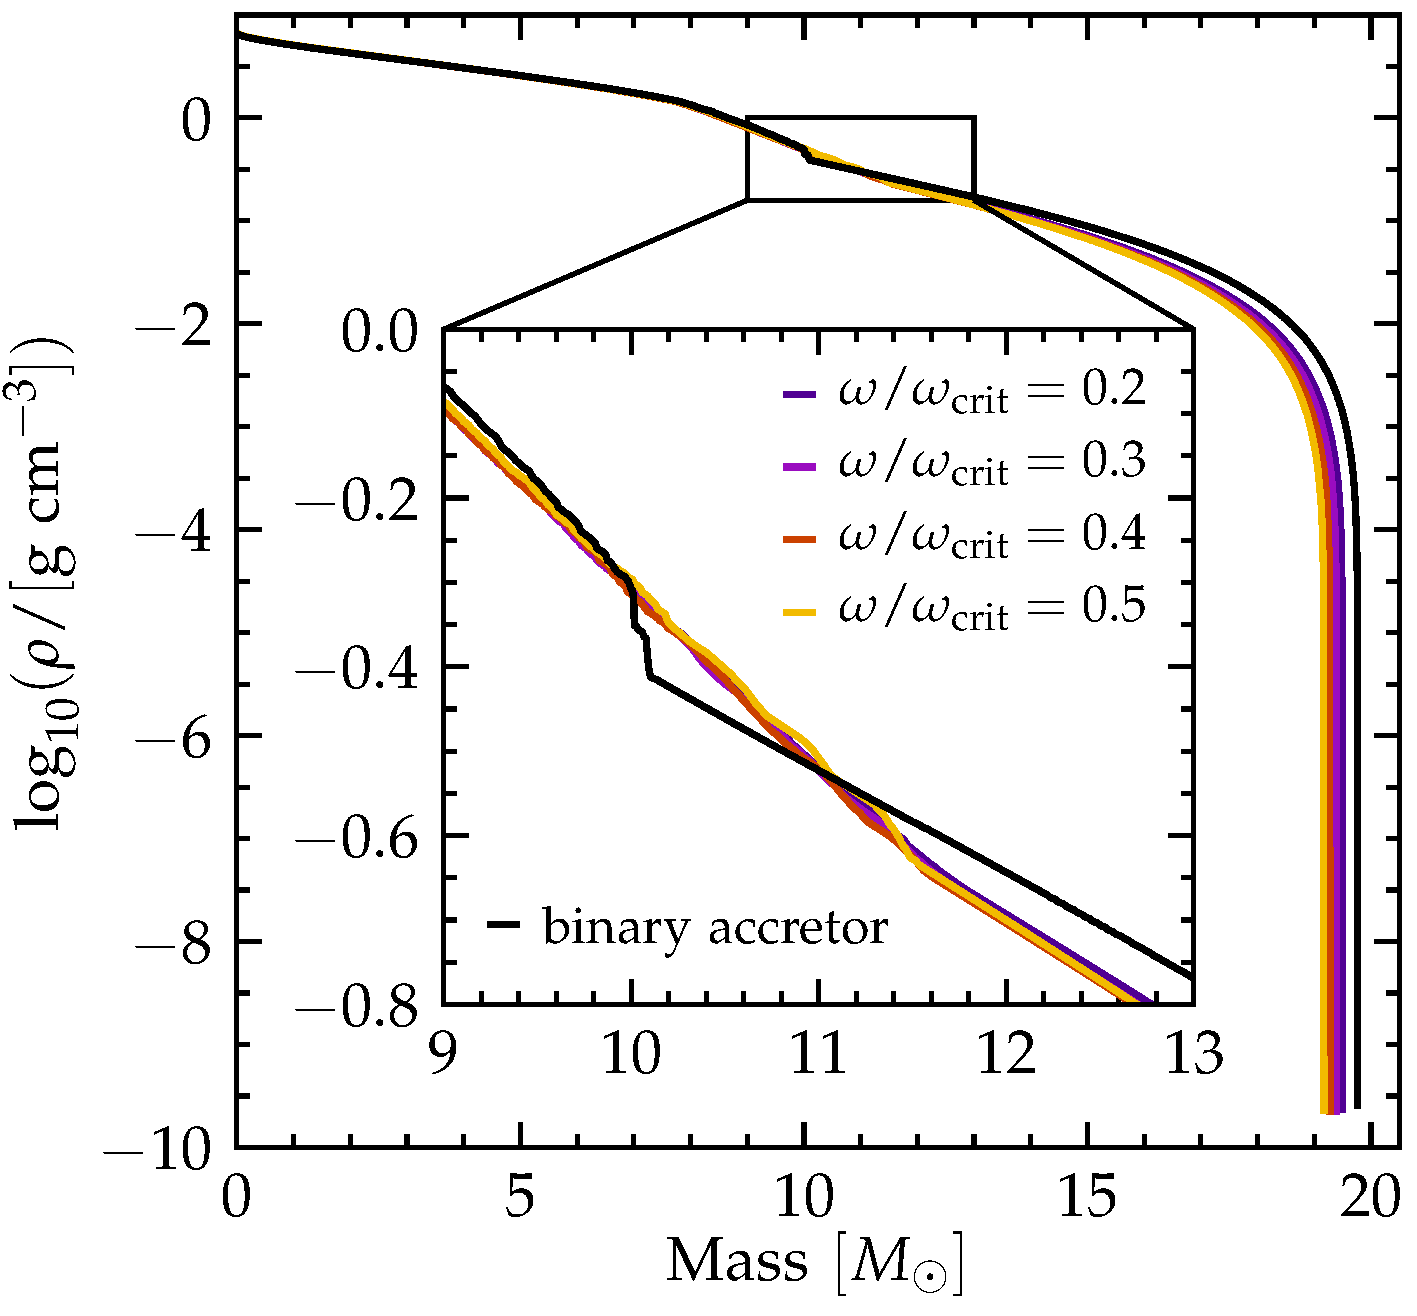
\includegraphics[width=0.47\textwidth]{rho_comparison}
  \caption{Comparison of the density profiles of the accretor model
    (black) and single $20\,M_\odot$ rotating stars (colors). The
    models are compared when they reach the same central H mass
    fraction of $X_c=0.085$ (point G in \Figref{fig:HRD_both} for the
    accretor). The inset magnifies the region above the core, where
    the outcome of common envelope events is decided. Because of the
    growth of the core, the density profile of the accretor in this
    region is significantly different.}
  \label{fig:rho}
\end{figure}

A convective layer above the hydrogen burning core that develops
during main-sequence evolution is uncommon for 20\Msun\ single star
models at Z=0.01 (see, e.g.,  \citealt{schootemeijer:19} for lower metallicity
and higher mass models showing off-center convective layers on the
main-sequence). Apart from impacting the composition and density
profile of the star, it is possible that it would also affect the
future evolution of the star.

To illustrate the effect of such off-center convective layer,
\Figref{fig:rho} shows a comparison of the density profiles between
the accretor model (point G in \Figref{fig:HRD_both}) and our four
initially $20\,M_\odot$ single rotating stars when they reach the same
central H mass fraction $X_c=0.085$. Convection
significantly alters the density profile above the core of the
accretor compared to a single star. The sharper inner density drop and
shallower density profile of accretors may be possible to explore with
asteroseismology: \zoph\ itself has been observed to show non-radial
pulsations \citep{walker:05}, which may be involved in the transient
appearance of emission lines and a decretion disk. If compared to a
star of comparable mass which evolved as single, the pulsations could
shed light on the structural differences between single stars and
binary products.

Moreover, for systems other than \zoph's progenitor, if the
binary remains bound after the explosion of the donor and the
evolutionary expansion of the accretor leads to a common envelope
\citep[e.g.,][]{paczynski:76}, the layer above the He core is crucial
to determine the success or failure of the common envelope
ejection. This might be
crucial for our understanding of gravitational wave
progenitors. Common envelope simulations have so far neglected the
impact of previous RLOF phase(s) on the density structure of the stars
initiating the dynamically unstable mass transfer.

\begin{figure*}[tbp]
  \centering
  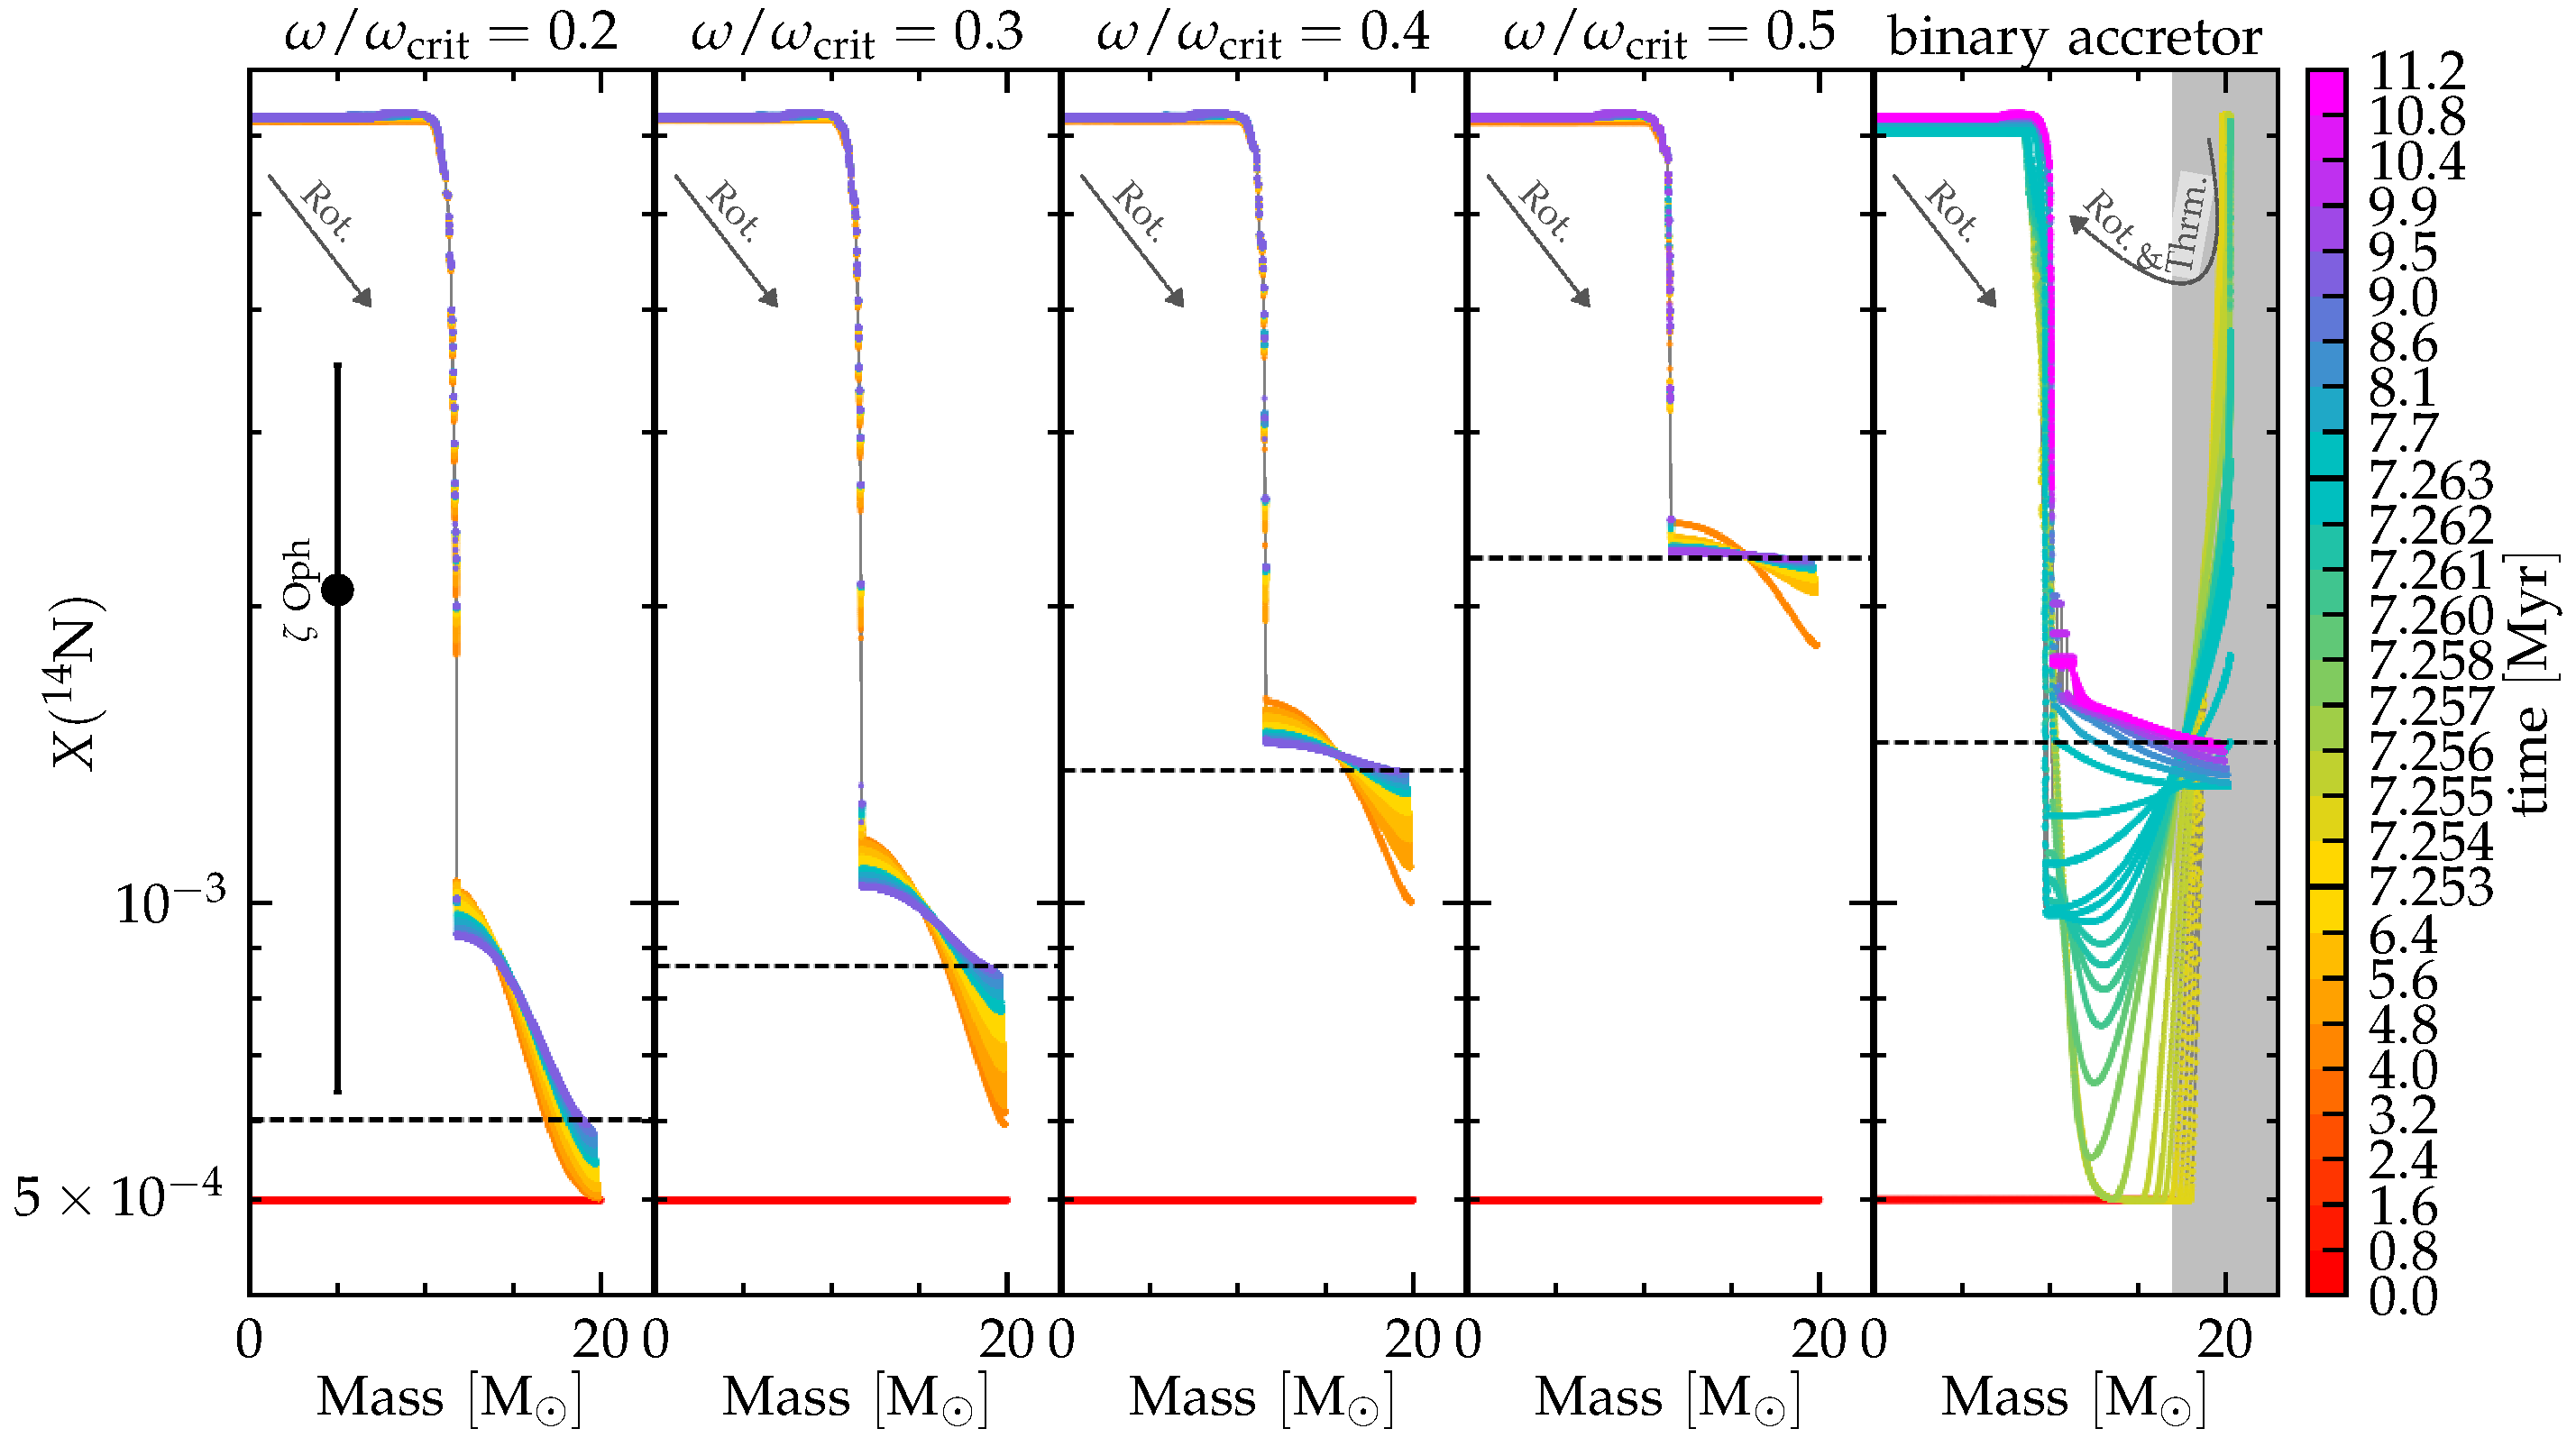
\includegraphics[width=\textwidth]{n14_colored} % struct_complete_zeta_ab
  \caption{$^{14}\mathrm{N}$ mass fraction as a function of mass
    coordinate for $20\,M_\odot$ single star models with increasing
    $\omega/\omega_\mathrm{crit}$ at birth (first four panels), and
    for the accretor of our fiducial binary (last panel). The colorbar
    is is non-uniform and allows for more color variation during
    RLOF. In each
    panel, the red flat line marks the primordial value for
    $Z=0.01$, the thin dashed black line marks the surface value at TAMS. In
    the last panel, the gray area highlights mass accreted during
    RLOF. The black errorbar in the first panel shows the surface
    $^{14}\mathrm{N}$ of \zoph\ estimated by \citetalias{villamariz:05} assuming
    the surface mass fraction of H from \Tabref{tab:surf_prop}. The
    abundance of $^{14}\mathrm{N}$ alone is not strongly
    constraining.
  }
  \label{fig:n14}
\end{figure*}

\subsection{Internal composition profile -- comparison to single stars}
\label{sec:mix_comparison_single}

We now compare the composition profiles in our accretor and in single
rotating massive star models. The first four panels of
\Figref{fig:n14} show the mass fraction of $^{14}\mathrm{N}$ as a
function of mass coordinate along the evolution of four $20\,M_\odot$
stars initialized with $\omega/\omega_\mathrm{crit}=0.2,0.3,0.4,0.5$.
The last panel of \Figref{fig:n14} shows our accretor model. While we
focus here on $^{14}\mathrm{N}$, \Figref{fig:composition_huge} shows a
similar plot containing also $^{12}\mathrm{C}$ and $^{16}\mathrm{O}$.

The first four panels of \Figref{fig:n14} show the typical rotational
mixing profiles: $^{14}\mathrm{N}$ rapidly rises by about an order of
magnitude in the core because of the CNO burning, and it is then mixed
outwards (as indicated by the arrows in the top left corner of each
panel). At any time the $^{14}\mathrm{N}$ profile is monotonically
decreasing with mass coordinate, and the higher the initial rotation,
the higher the surface $^{14}\mathrm{N}$ mass fraction reached at TAMS
because of the more efficient rotational mixing.

Conversely, the $^{14}\mathrm{N}$ mass fraction profile of the
accretor is \emph{not} monotonic throughout the evolution.  The
profile is shaped by two main processes: (i) accretion of
CNO-processed material from the donor star mixed inwards by meridional
circulations and thermohaline mixing (as indicated by the top right
arrow in the last panel), (ii) outward mixing of the CNO-processed
material from the accretor's core caused by rotational mixing -- as in
the single stars -- and rejuvenation.

Initially, the tidally synchronized accretor star rotates too slowly
($\lesssim 3\,\kms$) for significant outward rotational mixing out of
the core, and until the onset of RLOF (roughly at 7.25\,Myr) no
appreciable variation of the envelope $^{14}\mathrm{N}$ mass fraction
occurs. During late RLOF after the ``kink'' feature between C and D in
\Figref{fig:HRD_both}, N-enriched material from the donor's core piles
onto the accretor's surface -- inside the gray area. The
close-to-critical rotation (through Eddington-Sweet circulations) and
the inversion in the mean molecular weight $\mu$ (through thermohaline
mixing) drive inward mixing of the N-rich material and dilute it in
the envelope (see also \Figref{fig:D_mix}).

Simultaneously, the mere growth in mass causes the steepening of the
core-temperature gradient and increase in the convective core mass
\citep[rejuvenation, e.g.,][]{schneider:16}, driving some outward
convective mixing of N-rich material. The evolution of the structure
modified by accretion also causes the formation of an off-center
convective region (cf.~\Figref{fig:D_mix}) which persists at least
until TAMS, when we stop our model. Because the convective turnover
timescale is much shorter than the evolutionary timescales, convection
homogenizes the composition of this region and produces ``steps'' at
the outer edge of the core (slightly outside mass coordinate
10\,$M_\odot$).

\subsection{Comparison to \zoph's composition, radius, and rotation rate}
\label{sec:surf_comp}

    % this table was automatically generated using the table.ipynb in the repository associated to this manuscript
    \begin{table*}[hbpt]
    \centering
    \begin{tabular}{c|c|c|c|c|c|c|c|c}
    \hline\hline
    $M \ [M_\odot]$ & $R\ [R_\odot]$ & $\log_{10}(\omega / [\mathrm{s^{-1}}])$ & $v_\mathrm{rot} \ [\kms] $ & $X(^{1}\mathrm{H})$ & $X(^{4}\mathrm{He})$ & $X(^{12}\mathrm{C})$ & $X(^{14}\mathrm{N})$ & $X(^{16}\mathrm{O})$ \\
    \hline
    20.1 & 9.6 & -4.263 & 366.1 & 0.678010 & 0.312093 & 0.001344 & 0.001340 & 0.004148 \\
    \hline
    \end{tabular}
    \caption{Properties of the accretors shortly after the end of RLOF
    (last thin blue cross in \Figref{fig:HRD_both})}
    \label{tab:surf_prop}
    \end{table*}
    



In \Figref{fig:n14}, the black errorbar in the first panel shows
\zoph's surface $^{14}\mathrm{N}$ from \citetalias{villamariz:05}
(assuming the surface H mass fraction from our model listed in
\Tabref{tab:surf_prop}). The mass fraction of $^{14}\mathrm{N}$ alone
is not sufficient to distinguish between these models, and already a
moderate $\omega/\omega_\mathrm{crit}\geq0.3$ is sufficient for models
to reach the lower limit of the error bar.

\Tabref{tab:surf_prop} summarizes the surface properties of the
accretor star at 8.5\,Myr (fourth panel of \Figref{fig:D_mix}),
roughly corresponding to \zoph's position on the HR diagram
today. Both the mass and radius agree reasonably well with the
estimates from \citetalias{villamariz:05} and previous studies, that
is~$20\,M_\odot$ and $8.3\pm1.5\,R_\odot$, respectively. Our radius of
$9.8\,R_\odot$ is larger by $\sim0.6\,R_\odot$ than the equatorial
radius recently measured by \cite{gordon:18}, and our model has
$T_\mathrm{eff}\simeq31\,300$\,K, on the lower end of the range
considered by \citetalias{villamariz:05}. The surface
rotational velocity in excess of $350\,\kms$ is also in the correct
ballpark albeit possibly on the low end.

We report the surface H mass fraction\footnote{We obtain the mass
  fractions of individual elements inverting the definition
  $\varepsilon(X)=12+\log_{10}(N_X/N_H)$, where $N_X$ and $N_H$ are
  the number fractions of species $X$ and H, respectively
  \citep[e.g.,][]{lodders:19}.}, lower than primordial because of the
accretion of nuclearly processed material, and the surface mass
fraction of the most prominent species $^4\mathrm{He}$,
$^{12}\mathrm{C}$, $^{14}\mathrm{N}$, $^{16}\mathrm{O}$.  Assuming our
surface H mass fraction $X(^1\mathrm{H})$, the corresponding mass
fractions of $^4\mathrm{He}$, $^{12}\mathrm{C}$, $^{14}\mathrm{N}$,
$^{16}\mathrm{O}$ obtained by \citetalias{villamariz:05} are
$0.34^{+0.14}_{-0.05}$, $0.0006\pm0.0004$, $0.002\pm0.001$, and
$0.005\pm0.004$.

By the accretor's TAMS, rotational mixing (in the
form of Eddington-Sweet circulations) and thermohaline mixing nearly
homogenize the composition of the envelope of our accretor's
model. The surface mass fractions we obtain are sensitive to the
interplay between several poorly understood processes treated in one
dimension: mass accretion efficiency, rotationally enhanced wind mass
loss, thermohaline, and inward rotational mixing. These also impact
the composition of the envelope, and thus its radius and
$T_\mathrm{eff}$. Therefore, although not perfect, we consider the
match with the mass fractions reported by \citetalias{villamariz:05}
surprisingly satisfactory.

\section{Robustness of the models and discussion}
\label{sec:discussion}

Models of the interior evolution of stars require the use of several
poorly constrained parameters, most arising from the one-dimensional
representation of multi-dimensional phenomena (convection, mixing,
rotation, etc.). This remains true when modeling two stars in a
binary, with the added caveat that an even larger number of parameters
enters in the treatment of binary interactions (and in particular mass
transfer). This emphasizes the need for observational constraints and
motivated us to compare our models to the observationally well
characterized \zoph.

Accretor stars are expected in most populations of (massive) stars,
both in clusters \citep[e.g.,][]{chen:09, wang:20} and in the field
\citep[e.g.,][]{demink:11, demink:13}. However, these might not
obviously stand out as binary products in kinematics surveys
\citep[e.g.,][]{renzo:19walk}. Therefore, to inform the search for
accretor stars in observed samples, it is also necessary to
characterize the robustness of model predictions against numerical,
physical, and algorithmic choices.  In
\Secref{sec:single_star_uncertainties} we report on exploration of
parameter variations for each individual star in the binary and our
single star models. We
discuss parameters governing the binary evolution
\Secref{sec:bin_param}, and the consequences of the assumed SN
explosion of the companion in \Secref{sec:SN_comp}.


\subsection{Uncertainties in the single-star physics}
\label{sec:single_star_uncertainties}

\paragraph{Rotation}
% rotation and rotational mixing
Rotation is a critical ingredient of our models: it governs the
equatorial radius and thus $\omega/\omega_\mathrm{crit}$. Therefore,
by assumption, it also controls the mass transfer efficiency through
mechanical enhancement of the accretor's wind (see
\Secref{sec:bin_param}). Through Eddington-Sweet meridional
circulations, rotation affects outward mixing from the core, and more
importantly inward mixing from the surface.  We emphasize that the
shellular approximation used in one-dimensional stellar evolution
codes might not be appropriate for
$\omega/\omega_\mathrm{crit}\simeq 1$, which our accretor star reaches
during RLOF.  Decreasing the diffusion coefficient for Eddington-Sweet
meridional circulations by a factor of 10 has a very small effect on
the evolution of the accretor on the HR diagram. However, the
noisiness during the late RLOF phase (beyond point B in
\Figref{fig:HRD_both}) increases in amplitude, confirming that the
details of this part of the evolution are sensitive to the treatment
of rotational mixing (and its interplay with other processes).

\paragraph{Angular momentum transport}
% AM transport
Our models assume a Spruit-Tayler dynamo \citep{spruit:02} for the
transport of angular momentum throughout the evolution. Adopting the
stronger angular momentum transport from \cite{fuller:19} might result
in a more efficient spin-down of the surface during RLOF, possibly
allowing for more accretion of mass.

The accretor is spun up late and from the surface inwards. It also
reaches critical rotation in contrary to the single star models, which
are initialized at ZAMS with rigid rotation. Late during the mass
transfer, even the weak core-envelope coupling of \cite{spruit:02} is
sufficient for the accretor to achieve rigid rotation. Subsequently,
the envelope spins down because of wind mass loss and more importantly
the core spins significantly up because of its evolutionary
contraction. We expect that following \cite{fuller:19} the core would
lose more angular momentum to the envelope, limiting its ability to
spin up as it contracts and decreasing its rotational velocity.
Nevertheless, we expect that the difference with single star
rotational profiles would remain, albeit possibly smaller, because of
the shorter evolutionary time left.

\paragraph{Thermohaline mixing}
% thermohaline mixing
During RLOF, thermohaline mixing in the envelope becomes the dominant
mixing process. In \MESA, each mixing process is represented by its
own diffusion coefficient, and they are then summed together
\citep[e.g.,][]{paxton:11}, under the implicit assumptions that mixing
processes are independent from each other. This is typically
reasonable since locally one process dominates the mixing.  In the
envelope of our accretor model, initially Eddington-Sweet circulations
are dominant, however thermohaline mixing reaches and exceeds their
diffusivity late during the mass transfer because of accretion of
chemically enriched material from the donor. If fast rotation can
physically modify thermohaline mixing processes, this could impact our
accretor models. We also computed models with enhanced efficiency of
thermohaline mixing \citep[a factor of 100 higher,
][]{schootemeijer:19}, but these proved numerically unstable when
accreting CNO-processed material.

\paragraph{Convective overshooting}
On the basis of nucleosynthesis arguments \citep[e.g.,][]{herwig:00}
and asteroseismology \citep[e.g.,][]{moravveji:16}, an exponentially
decreasing overshooting is generally considered
preferable. Nevertheless, we have also explored models with a
step-function overshooting from \cite{brott:11}. Our fiducial
exponential overshooting was chosen to reproduce the width of the
main sequence of the models of \cite{brott:11} and, not-surprisingly,
the qualitative evolution of our fiducial model and models with step
overshooting is similar. However, adopting a step overshooting
provides a higher diffusivity at the outer edge of the core (cf.\
exponential decrease), which ultimately impacts the details of the
chemical profile at the outer edge of the core, and the morphology of
the evolutionary tracks during late RLOF.

\paragraph{Stellar winds}
\zoph\ is one of the low-luminosity O-type stars for which
\cite{marcolino:09} found a lower-than-predicted wind mass loss rate.
To address the ``weak wind problem'', we also attempted running models
with artificially decreased wind mass loss rate
\citep[e.g.,][]{renzo:17}, but these resulted in super-critically
rotating ($\omega/\omega_\mathrm{crit}>1$) post-RLOF accretor stars
with untrustworthy numerical results. The solution to the ``weak wind
problem'' is not currently known, but \cite{lucy:12} and
\cite{lagae:21} suggest that observed mass loss rates might be
underestimated, suggesting that the theoretically motivated hot star
wind mass loss rate might still be appropriate to model low luminosity
O-type stars.

Our models use the \cite{vink:00} mass-loss rate on the main sequence,
which includes the enhancement due to the bistability jump at
$T_\mathrm{eff}\simeq25\,000\,\mathrm{K}$. This results in the
dramatic increase in the surface spin down at late times in
\Figref{fig:surf_rot}. However, the mass-loss (and consequently
spin-down) enhancement at the bistability jump has recently been
questioned by \cite{bjorklund:21}. If such enhancement does not occur,
it is possible our models would retain a higher surface rotation rate,
and higher $\omega/\omega_\mathrm{crit}$. This would influence in a
similar way our single star models and our accretor, suggesting the
relative comparison between these models would still remain valid.

\paragraph{Metallicity}
%metallicity
Throughout this study, we assumed an initial metallicity $Z=0.01$
informed by the asteroseismology of low mass stars in
Upper-Centaurus-Lupus \citep[e.g.,][]{murphy:21}, identified as the
parent association for \zoph\ by \cite{neuhauser:20}. Moreover, we
have assumed that mass fractions of each element scale with the Solar
values \citep{grevesse:98}, which might not be appropriate especially
for massive stars \citep[e.g.,][]{grasha:21}. With these assumptions,
the initial mass fraction of $^{12}\mathrm{C}$ and $^{14}\mathrm{N}$
are lower than the values reported by \citetalias{villamariz:05} for
\zoph. Even though both values increase during mass transfer, our
model still slightly under-predicts them. Improved agreement could be
obtained changing the ratio of abundances to non-solar values, or by
changing the efficiency of downward rotational and thermohaline mixing
which dilutes the accreted material into the secondary's envelope.

We also ran a model identical to the one described in
\Secref{sec:best_model}, except with $Z=Z_\odot=0.0142$
\citep{asplund:09} with the same composition scaling from
\cite{grevesse:98}.  Qualitatively, the binary evolution remains
similar, with the higher metallicity stars having slightly larger
radii and cooler $T_\mathrm{eff}$ at a given luminosity. This still
produces a stable case B RLOF, however, matching the high present-day
$T_\mathrm{eff}=32\,000\pm2\,000$ of \zoph\ (e.g.,
\citetalias{villamariz:05}) requires more massive and hotter accretors
at higher $Z$ (see also \Secref{sec:bin_param}).

\subsection{Uncertainties in the treatment of mass transfer}
\label{sec:bin_param}

\paragraph{Mass transfer efficiency, $\beta_\mathrm{RLOF}$}
We regulate the accretion efficiency through the rotational
enhancement of mass loss \citep[e.g.,][]{langer:98}.  However, whether
critical rotation can effectively stop the accretion of matter is
unclear. \cite{popham:91} and \cite{paczynski:91} argued that
accretion of mass (but not angular momentum) might be possible even at
or beyond critical rotation.

During RLOF, the total amount of mass lost by the donor is
$\Delta M_\mathrm{donor} \simeq 10.6\,M_\odot$, of which only
$\Delta M_\mathrm{accretor}\simeq 3.4\,M_\odot$ are successfully
accreted by the companion. This corresponds to an overall mass
transfer efficiency
$\beta_\mathrm{RLOF}\equiv |\Delta M_\mathrm{accretor}|/|\Delta M_\mathrm{donor}| \simeq 0.32$,
although the accretion efficiency is \emph{not} constant throughout
the mass transfer \citep[e.g.,][]{vanrensbergen:06}. In our models,
the mass transfer efficiency depends on the radial and rotational
evolution of the accreting star. During RLOF, the accretor is out of
gravothermal equilibrium with significant impact on its radius and
ultimately on the amount of mass transferred and its angular
momentum. In reality, the gas stream between the two stars, the
hot-spot due to the RLOF stream hitting the accretor's surface (see
below), and the geometric distorsion of the outer layers because of
the centrifugal forces would not follow the spherical symmetry imposed
by 1D codes such as \texttt{MESA}.

While the mass transfer efficiency, $\beta_\mathrm{RLOF}$, and
importantly its time-evolution need further attention, it is also
likely that this parameter and its evolution depend on the details of
the system (masses, mass ratio, period, etc.). For instance, to
explain the lower mass sdO+Be binaries found by \cite{wang:21_sdOBe}
it is likely that a larger mass transfer efficiency would be
required. Conversely, \cite{petrovic:05} argued for
$\beta_\mathrm{RLOF}\simeq 0.1$ to reproduce WR+O star binaries.


Most studies, especially using rapid population synthesis tools,
typically assume a constant $\beta_\mathrm{RLOF}$ and neglect the
out-of-equilibrium phase of the accretor and how this can impact the
binary and orbital evolution. Alternatively, rapid population
synthesis can limit the accretion rate based on the thermal timescale
of the accretor (calculated from models in gravothermal
equilibrium). Based on this approach, \cite{schneider:15} found a
higher $\beta_\mathrm{RLOF}\simeq 0.7$ for a binary comparable to ours
(initially $M_1=20\,M_\odot$, $M_2=0.7M_1$ with separation
$a\simeq300\,R_\odot$), although their $\beta_\mathrm{RLOF}$ is very
sensitive to the initial mass ratio and period in this regime.

\paragraph{Specific angular momentum of accreted material}
% Another free parameter in the treatment of mass transfer is the
% specific angular momentum of the accreted material.
This is an uncertain quantity and likely depends on the geometry of
the accretion process, and in particular, whether the accretion stream
through the first Lagrange point (L1) hits the accretor star directly,
or if instead an accretion disk is formed \citep[e.g.,][]{demink:13}.

We calculate the minimum distance $R_\mathrm{min}$ between the stream
coming from L1 and the accretor using the fit from \cite{ulrich:76} to
the numerical results of \cite{lubow:75}. We find
$R_\mathrm{min}\simeq 1.5\,R_\odot < R_\mathrm{accretor}$: this
suggests that the stream should hit the accretor directly, without
forming an accretion disk. Nevertheless, for the sake of numerical
stability, we assume the incoming material and the stellar surface to
have the same specific angular momentum. This provides a slow angular
momentum accretion and consequent spin-up of the surface.

For a more physically motivated approach, we also attempted
calculations using for specific angular momentum of the accreted
material $j=\sqrt{1.7GM_\mathrm{accretor}R_\mathrm{min}}$,
representative for direct impact of the incoming stream with the
accretor \citep{lubow:75}. This is typically much larger than the
specific angular momentum of the accretor's surface. However, these
models proved numerically more unstable and providing less trustworthy
results after the accretor is spun up significantly. In general,
allowing for a faster accretion of angular momentum results in a
faster spin-up, and a lower overall mass transfer efficiency
$\beta_\mathrm{RLOF}$.

\paragraph{Specific entropy of the accreted material}
In our models, the composition of the transferred material is
determined by the structure of the donor and the mass transfer rate
calculated following \cite{kolb:90}, but we need to specify its
specific entropy when it reaches the accretor surface. We follow the
common practice of assuming the specific entropy of the incoming
material to be same as the accreting surface. The scenario justifying
this hypothesis is that during RLOF the matter is sufficiently
optically thin so that radiative processes can rapidly equalize the
entropy between the RLOF stream and the accreting surface. However,
the very large mass-transfer rates we find (cf.~\Figref{fig:MT}) might
result in optically thick flows for which this approximation might not
be appropriate.

\paragraph{Rejuvenation and core growth}
Because of the increase in mass, our accretor star is rejuvenated: its
total main-sequence lifetime is longer than the lifetime of a single
star born with the final post-RLOF mass of the accretor\footnote{But
  not significantly longer than the lifetime of a single star of its
  initial, pre-RLOF mass.}  \citep[e.g.,][]{schneider:16}. The
rejuvenation is due to the increase - in mass - of the core region,
which brings fresh nuclear fuel inwards. Our results are in agreement
with \cite{hellings:83}, while \cite{braun:95} did not find any
rejuvenation in their accretor models. We attribute this difference to
the lack of convective boundary mixing (e.g., overshooting, efficient
semiconvection, shear) in their models, which impedes the growth of
the core. In our models, the growth of the core is initially driven by
convection and overshooting, and to a lesser extent by dynamical
shear, while the off-center convective layer of \Figref{fig:D_mix} and
\Figref{fig:rho} does not contribute significantly to the inward
mixing of H-rich material and the rejuvenation itself. We cannot
exclude that in the presence of a strong shell undershooting that
convective layer would also mix efficiently with the core, enhancing
further the rejuvenation effect


\paragraph{Initial binary parameters}
The initial donor mass $M_1$, mass ratio $q\equiv M_2/M_1$, and the
period of the progenitor binary of \zoph\ cannot be directly
constrained from observations. We have explored variation in these,
and the qualitative behavior of the models is similar.  Shorter
initial periods results in larger post-RLOF orbital velocities, and
thus larger runaway velocities if the binary is disrupted at the first
SN (see \Secref{sec:SN_comp}). For example, taking $P$=75\,days (cf.\
100\,days in our fiducial model), the binary still experiences stable
case B mass transfer, but the post-RLOF orbital velocity of the
accretor is about $60\,\kms$, that is $\sim{}10\,\kms$ higher than in
our fiducial model, because of the larger orbital velocity in the
tighter binary system.

Increasing the donor mass also has a similar effect on the post-RLOF
orbital velocity of the accretor. Using $M_1=30\,M_\odot$ (cf.\
$25\,M_\odot$ in \Secref{sec:best_model}), $M_2=17\,M_\odot$, and
$P$=100\,days, we obtain a post-RLOF velocity of $65\,\kms$. However,
this produces a stripped donor of $\sim$16\,$M_\odot$ at RLOF
detachment, with stronger wind mass loss rate. Therefore this binary
is expected to widen relatively more than our fiducial model of
\Secref{sec:best_model}, slowing down the accretor. The increased mass
of the stripped donor star could also imply a lower chance of
exploding for the donor, which might instead collapse to a black-hole
(however, see \Secref{sec:SN_comp}).

The higher $M_1$ does not significantly change the post-RLOF total
mass of the accretor, with $M_2$ remaining about $\sim$20.5\,$M_\odot$, since
in our models accretion is regulated mostly by the spin up of the
accretor, and we do not couple the specific angular momentum of the transferred
material to the orbit or the donor's spin.

However, changing the initial mass ratio also changes the difference
between the main-sequence lifetime of the two stars, and thus how far
along the main sequence the accretor is at the onset of RLOF. The
observed position of \zoph\ on the HR diagram, particularly its
relatively high $T_\mathrm{eff}$, is difficult to reproduce assuming
initially less massive accretors (which would remain too cool even
after accreting mass), or a more equal initial mass ratio (which would
produce an accretor that is too evolved and cool at the onset of mass
transfer).


\subsection{The explosion of the donor star}
\label{sec:SN_comp}

Throughout this study, we have assumed the ``binary SN scenario'' to
explain the runaway nature of \zoph: after the mass transfer phase,
the explosion of the donor disrupts the binary and ejects the accretor
at roughly its pre-explosion orbital velocity
\citep[e.g.,][]{blaauw:61, renzo:19walk}. This fate occurs to the
majority of massive binary systems, and \zoph\ might be the best
example of it \citep[e.g.,][]{blaauw:52, blaauw:61,
  hoogerwerf:00}. \cite{neuhauser:20} suggested not only the companion
successfully exploded producing the pulsar PSR B1706-16 and ejecting
\zoph, but also that the explosion produced radioactive
$^{60}\mathrm{Fe}$ which polluted Earth.

From kinematic and orbital considerations they estimated the pulsar
received a natal kick of $253\pm54\,\kms$, which would be sufficiently
large to unbind the binary which has
$v_\mathrm{orb}=\sqrt{G(M_1+M_2)/a}\simeq 135\,\kms$ at the end of our
binary simulation (blue diamond in \Figref{fig:HRD_both}), and this
will decrease further in the remaining time to the donor's
core-collapse \citep{kalogera:96, tauris:15}.

The SN ejecta mass would depend on the post-RLOF wind mass loss of our
donor star, which is uncertain \citep[see also][]{renzo:17, vink:17,
  gilkis:19, sander:20}. At the end of our binary evolution simulation, our
stripped donor is $\sim{}9.4\,M_\odot$, with a surface H fraction of
$X\lesssim0.2$ for a layer of $\Delta M \simeq 2.5\,M_\odot$.  Its
wind mass-loss rate is $\sim10^{-5}\,M_\odot \mathrm{yr^{-1}}$,
calculated assuming the empirical Wolf-Rayet wind mass loss
prescription from \citet[][see also \Figref{fig:MT}]{nugis:00}. We
expect that the donor will explode in a H-free type Ib
supernova. Although our stripped donor is rather massive, recent
studies hints at a higher ``explodability'' of donor stars in binary
systems \citep[e.g.,][]{schneider:21, laplace:21, vartanyan:21}.

We have neglected the impact of the explosion on the structure of the
accretor star. At the time of the explosion, the accretor subtends a
solid angle $\sim{}R^2/a^2\simeq 2\times10^{-3}$\,steradians with $R$
the accretor radius and $a$ the binary separation. We neglect the
post-RLOF wind-driven orbital widening for this estimate.  The blast
wave will hit the accretor causing mass loss -- directly via ablation
and by injecting energy in the envelope, inflating it and enhancing
its wind \citep{wheeler:75, tauris:98, podsiadlowski:03, hirai:18, ogata:21}.
Because of the SN shock, the just ejected new runaway star might
appear bloated and redder (long before it overtakes the slowing SN
remnant). The impact of this brief out of thermal equilibrium phase on
the stellar spin should be investigated further.

Using 2D hydrodynamic simulations of the star-SN ejecta interactions
in close binaries ($a\lesssim 60\,R_\odot$,
cf. $a\gtrsim 343\,R_\odot$ in our fiducial binary model),
\cite{hirai:18} and \cite{ogata:21} found that the companion star recovers its
pre-explosion luminosity and effective temperature within a few years
to decades, and the amount of mass removed by the SN shock is
$\lesssim10^{-2}\,M_\odot$.  The SN ejecta might also pollute the
surface of the runaway by depositing processed nuclear material
\citep[e.g.,][]{przybilla:08, suda:21}. However, for the large final
separation of our model, little pollution is expected and enhanced
mass loss and inward mixing might quickly dilute any signature below
detectable levels.



\section{Summary \& conclusions}
\label{sec:conclusions}

The impact of mass transfer on the structure and evolution of accretors
stars in massive binaries has received relatively little attention in
the literature. To investigate this, we have performed \texttt{MESA}
calculations of massive binaries evolving two coupled stars
simultaneously.

As a first application, we focused on finding a model in which the
accretor properties are in qualitative agreement with observations of
the nearest O-type star to Earth. This is the runaway star \zoph, which has
long been suggested to be a former accretor star ejected from a binary
at the core-collapse of the donor star \citep[binary SN
scenario,][]{blaauw:61}. However, our models are also informative for
the generic population of massive stars accreting in binaries.


\subsection{Reproducing \zoph}

We found that the main features of \zoph\ can be
reasonably well reproduced using standard stellar physics
assumptions for the treatment of mass transfer, chemical mixing, and
rotation. Our choices are described in \Secref{sec:methods} and
Appendix~\ref{sec:software}.

Our fiducial model is a binary starting
with $M_1=25\,M_\odot$, $M_2=17\,M_\odot$, and $P=100$\,days at
metallicity $Z=0.01$ (see \Secref{sec:best_model}). This binary
experiences stable thermal-timescale Roche lobe overflow after the end
of the main sequence of the donor (case B).

The accretor compares well with observations of \zoph\ about
$1.5-2$\,Myrs after the end of mass transfer, corresponding to the
remaining donor's lifetime at the end of our simulations plus the
kinematic age of \zoph. Specifically, the position on the HR diagram
(cf.~\Figref{fig:HRD_both}), the runaway space velocity (estimated
based on the accretor's orbital velocity), the surface composition and
rotational velocity (cf.~\Tabref{tab:surf_prop}) are in the right
ballpark.

Our model of \zoph\ differs significantly from previous studies: in
contrast with the accretor models of \cite{vanrensbergen:96}, in our
model the $^{14}\mathrm{N}$- and $^4\mathrm{He}$-rich surface
composition is not the result of pure outward rotational mixing.
Instead, this material is transferred from the receding core of the
donor star and mixed from the surface inwards into the accretor by
meridional circulations and more importantly thermohaline mixing.
Thus, the present day surface mass fractions of \zoph\
constrain the mass transfer efficiency and mixing in the accretor. Our
results suggest \zoph\ should not be used to calibrate models of
rotational mixing in single star models.

We emphasize that the surface composition alone would not be a
smoking-gun of a past in a binary, especially given the large
uncertainties in the treatment of rotation and mixing in stellar
evolution models. In our models, the accretion of $^{14}\mathrm{N}$
from the donor star allows the accretor star to be simultaneously fast
rotating and $^{14}\mathrm{N}$-rich. Alternative scenarios where
\zoph\ evolved as a single, fast-rotating star require ad-hoc
explanations for the runaway velocity, and have been shown by
\citetalias{villamariz:05} to struggle in reproducing surface mass
fractions, apparent age, mass, and rotation rate simultaneously.

The surface rotation rate of the accretor post-mass-transfer is always
higher than the rotation rate of single stars initialized with
half-critical rotation, but might still be on the low side compared to
\zoph. However, the wind spin down might be overestimated in our
models (weak wind problem, cf.\ \citealt{marcolino:09, lucy:12, lagae:21}).

We also tested the
robustness of our fiducial model against variations in the initial parameters
and algorithmic representation of physical phenomena, discussed in
\Secref{sec:discussion}. Less massive accretors remain too cool
throughout the evolution to be compatible with \zoph, and initial mass
ratios closer to unity lead to a more evolved accretor at the onset of
mass transfer, again resulting in too cool temperatures. Increasing
the donor's initial mass might result in stripped stars unlikely to
form a neutron star in their final SN explosion.

\subsection{Accretors are not single rotating stars}

Our models also highlight some general differences between accretors in massive
binaries and stars evolving as single throughout their life. These
%have been so far under-appreciated but
might be important for several
sub-fields of astrophysics, including asteroseismology, stellar
populations, and time-domain and gravitational waves observations.

The first notable difference we find is the internal rotation
profile. Single rotating stars are usually initialized as rigid
rotators at birth, and throughout their evolution they spin down due
to wind mass loss. Conversely, accretors are spun up later during
their main-sequence evolution and from the surface inward. Moreover,
for single stars, the maximum rotation rate, that is the one assumed
at the beginning of the evolution, is poorly understood theoretically
and observationally \citep[e.g.,][]{ramirez-agudelo:13,
  ramirez-agudelo:15}. Conversely, accretors in binaries reach
critical rotation $\omega/\omega_\mathrm{crit}\simeq 1$
\citep[e.g.,][]{packet:81}. The later spin-up and higher achieved
rotation rate allow the accretor star to remain a fast rotator until
the end of its main sequence.

The angular momentum accreted at the surface of the accretor is
transported into the core (by the Tayler-Spruit dynamo in our
simulations). This results in a much faster rotating helium core at
the end of the main sequence compared to single stars. Such a fast
spinning helium core has potential implications for the final
explosion and the resulting compact object born from the accretor star
in an interacting binary system.

Finally, in our models, the accretion of mass leads to rejuvenation
and also the formation of a off-center convective layer above the
main-sequence core (cf.\ \Figref{fig:D_mix}). The latter ultimately
results in a sharper density drop at the core edge (cf.\
\Figref{fig:rho}), and a flatter density profile close to the end of
the main sequence. If physical, the presence of such a convective
layer could in principle be probed using asteroseismology. Depending
on how the accretor (and the binary) evolves in the future, this
difference could be crucial in determining the outcome of common
envelope events between massive stars and compact objects.\\


Improving our understanding of the evolution of the initially less
massive stars in massive binary systems is crucial for the upcoming
large surveys, stellar kinematics, and for the understanding of the
evolution of gravitational-wave progenitors in isolated
binaries. Although presently single, the nearest O-type star to Earth,
\zoph, can be used as an anchor point for the modeling of
accretors. Our models demonstrate that a broad agreement with
observations can be achieved with standard stellar evolution
assumptions. Future efforts should extend these models to a wider
mass, period, mass ratio, and metallicity range to investigate the
impact of binary evolution on the life, explosion, and after-life of
the secondary stars in massive binary systems.

\software{
  \MESA\ \citep{paxton:11,paxton:13,paxton:15,paxton:18,paxton:19},
  \texttt{mesaSDK} \citep{mesasdk},
  \texttt{ipython/jupyter} \citep{ipython},
  \texttt{matplotlib} \citep{matplotlib},
  \texttt{mesaPlot} \citep{mesaplot},
  \texttt{NumPy} \citep{numpy}.
}

\acknowledgements{We are grateful to E.~Zapartas, A.~Jermyn,
  M.~Cantiello, R.~Neuh\"auser, B.~D.~Metzger, S.~Oey, and S.~Justham
  for helpful discussions and feedback. We also thank P.~Marchant for
  helpful guidance with the newe superadiabaticity reduction
  capabilities in \texttt{MESA}. Support for this work was provided by
  NASA through the NASA Hubble Fellowship Program grant
  \#HST-HF2-51457.001-A awarded by the Space Telescope Science
  Institute, which is operated by the Association of Universities for
  Research in Astronomy, Inc., for NASA, under contract NAS5-26555.}

\appendix

\section{\texttt{MESA} setup}
\label{sec:software}

We use \code{MESA} version 15140 to compute our models.  The
\code{MESA} equation of state (EOS) is a blend of the OPAL \citet{Rogers2002}, SCVH
\citet{Saumon1995}, PTEH \citet{Pols1995}, HELM \citet{Timmes2000},
and PC \citet{Potekhin2010} EOSes.

OPAL \citep{Iglesias1993, Iglesias1996} provides the main radiative
opacities, with low-temperature data from \citet{Ferguson2005} and the
high-temperature from \citet{Buchler1976}. Electron conduction
opacities are from \citet{Cassisi2007}.

Nuclear reaction rates are a combination of rates from NACRE
\citep{Angulo1999}, JINA REACLIB \citep{Cyburt2010}, plus additional
tabulated weak reaction rates \citet{Fuller1985, Oda1994,
  Langanke2000}. Screening is included via the prescription of
\citet{Chugunov2007}.  Thermal neutrino loss rates are from
\citet{Itoh1996}. We use a
22-isotope nuclear network (\texttt{approx\_21\_plus\_cr56}).

The inlists, processing scripts, and model output are available at~\url{https://doi.org/10.5281/zenodo.4701565}.

\section{Resolution tests}
\label{sec:res_tests}


\begin{figure*}[htbp]
  \centering
  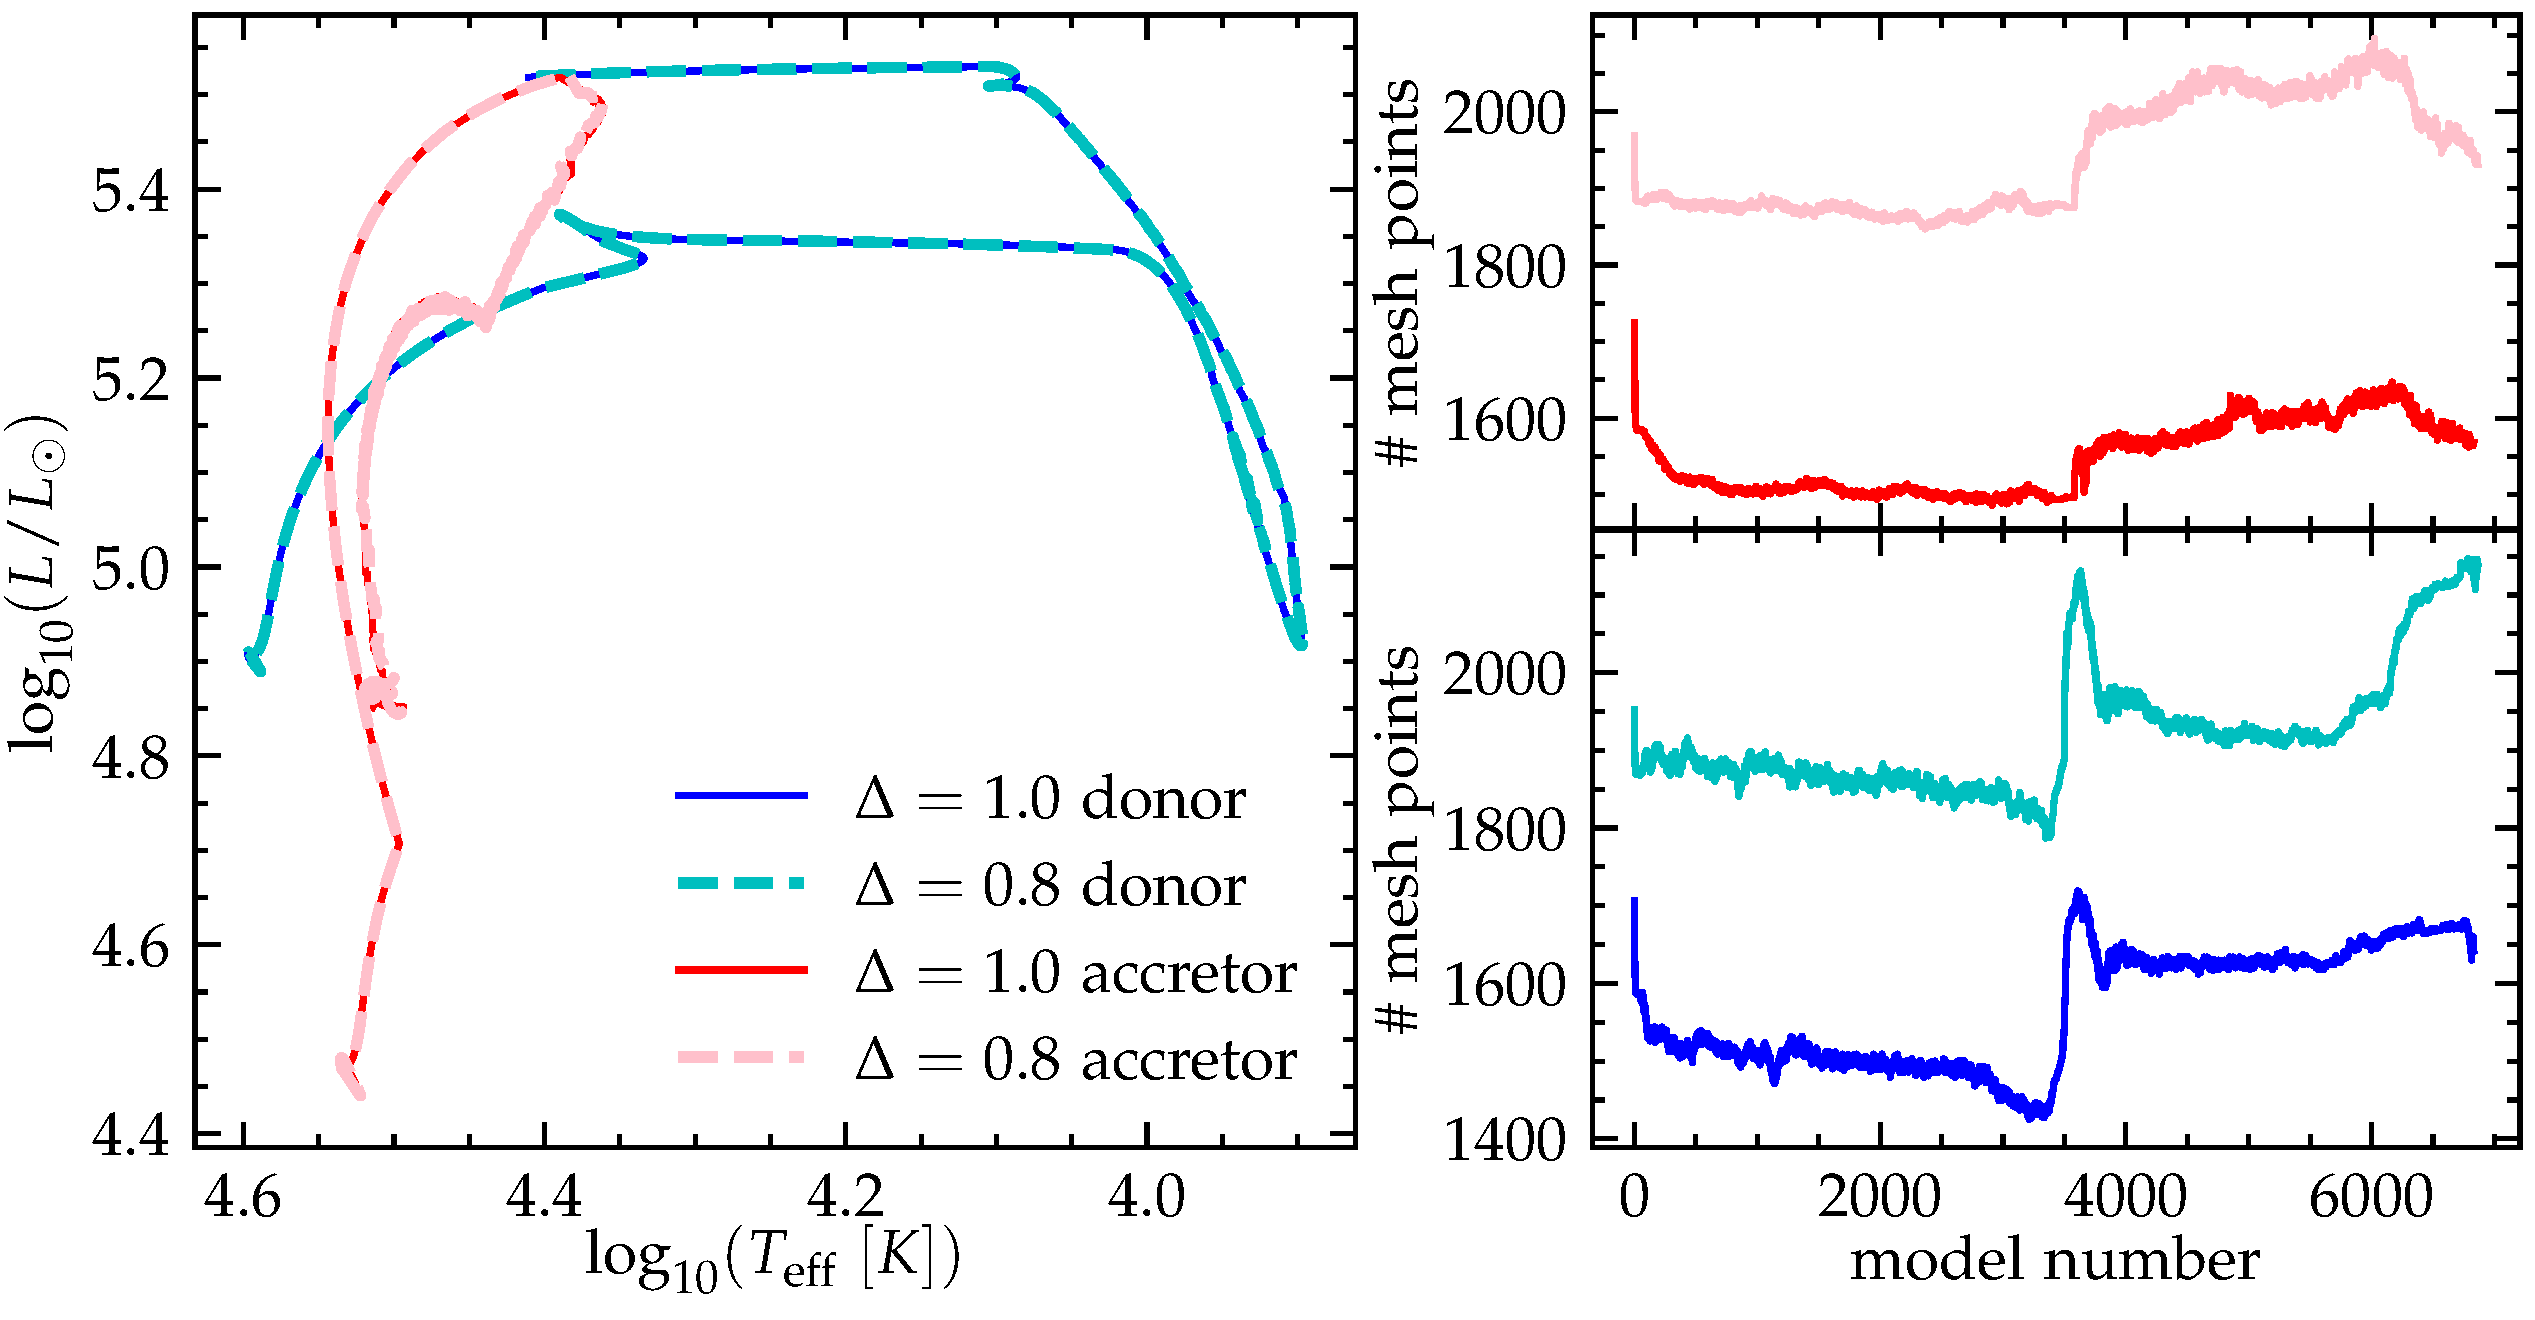
\includegraphics[width=\textwidth]{spatial_res_plot}
  \caption{Left: HR diagram comparison for our fiducial binary model varying
  the number of mesh points. We only show the evolution until our definition
  of RLOF detachment. Right: number of mesh points as a
  function of timestep number. In both panels, the blue/cyan tracks show the donor stars, the
red/pink tracks show the accretor. Thicker dashed lines correspond to
the models at higher resolution (i.e., lower $\Delta$ which indicates
the value of \texttt{mesh\_delta\_coeff}).}
\label{fig:sp_test}
\end{figure*}

We extensively checked the numerical convergence of our stellar
evolution calculations with increasing number of mesh
points. \Figref{fig:sp_test} shows that all the main features described
here do not vary when increasing the spatial resolution by increasing
the number of mesh points (i.e.,
decreasing \texttt{mesh\_delta\_coeff}). The right panel shows the
number of mesh points for the accretor (top) and donor (bottom) as a
function of the model number (akin to an arbitrary time
coordinate). About $\sim$7000 \texttt{MESA} timesteps are used to compute
the binary evolution. The higher resolution run has $\sim 20\%$ more
mesh points. The left panel shows the evolution on the HR diagram until the
detachment of the binary for the two accretor models (pink/red) and
the two donor models (blue/cyan).

Similarly, we tested the numerical convergence with decreasing
timestep size. This can be done decreasing the parameter
\texttt{mesh\_time\_coeff}. However, we were unable to successfully
compute models at higher temporal resolution. Partial results show a
good agreement with our fiducial model until \texttt{MESA} becomes
unable to find a satisfying numerical solution to the stellar
structure equations (typically
during RLOF). Lower temporal resolution models showed a similar
qualitative agreement but increased noisiness during the late RLOF
phase. For our fiducial model the adaptive timestep size never exceeds
$10^{3.8}$\,years with typical pre-RLOF timesteps of the order of $10^{3.2}$\,years
and sub-decade (occasionally sub-year) during RLOF. The main factor limiting the timestep
sizes is the change of surface angular momentum in both stars during
the mass transfer.


\section{Internal composition profile evolution}
\label{sec:X_fig}


\Figref{fig:composition_huge} compares the internal evolution of the composition
profile of single rotating stars with our accretor model.
We show mass fractions of $^{12}\mathrm{C}$  and $^{16}\mathrm{O}$ to complement the
mass fraction of $^{14}\mathrm{N}$ shown in \Figref{fig:n14}, and
reproduced also in the middle panel of \Figref{fig:composition_huge}.


\begin{figure*}[htbp]
  \centering
  \includegraphics[width=\textwidth]{huge_composition_colored}
  \caption{Same as \Figref{fig:n14}, but for $^{12}\mathrm{C}$ (top
    panel), and $^{16}\mathrm{O}$ (bottom panel). The first four
    panels show single rotating stars of initially $20\,M_\odot$, the
    rightmost panel shows the accretor in our fiducial binary. The middle panel is
    exactly the same as \Figref{fig:n14}. The red lines mark the
    initial mass fractions, black dashed lines indicate the TAMS surface mass
    fraction, and the black error bars in the first column indicate
    the surface composition of \zoph\ inferred by \citetalias{villamariz:05}
    using the surface H mass fraction from our model.}
  \label{fig:composition_huge}
\end{figure*}

\bibliographystyle{aasjournal}
\bibliography{./zeta_ophiuchi.bib}


\end{document}

%%% Local Variables:
%%% mode: latex
%%% TeX-master: t
%%% End:
